\chapter{Modular Robot configurations and gaits}
\label{config_gait}

\section{Modular Robot configurations}
\label{config}

Modular robots have the versatile capability of being able to reconfigure themselves, adapting to the environment and the task they must perform. They could, For example, be configured as a legged robot to step over an obstacle and then reconfigure to a snake robot to travel along a pipe. This ability renders them very useful in unknown and unstructured environments, where they excel other mobile robots.\\

In order to be studied, this variety of possible configurations require a classification, since the locomotion gaits that each configuration is able to perform and how to perform them change notably among the different configurations. The controller also varies with the configuration, and more complex configurations, such as legged ones, require more complex controllers to deal with coordination between all the limbs, between the limbs and body and in general, between all their joints to achive a optimal gait.\\

\subsection{Classification by the arrangement of their basic unit}
\label{config_basic_unit}
One common way of classifying the different types of modular robots and their configurations is to base it on the arrangement of their basic unit, classfying them in lattice type, chain type, or hybrid type.\\

\emph{Lattice} modular robots have their modules arranged in some regular pattern along 3D space, resembling atoms in crystals and their configurations are usually described using crystallographic displacement groups. These kind of lattice structures are computationally simpler to describe, and their reconfiguration planning can be scaled easier to more complex systems. In fact, locomotion in this kind of modular robots is achieved by reconfiguration, changing the position of individual modules in that lattice in such a way that the global position of the modular robot is displaced towards the goal position. 
\\

Some examples of modules that can be classified as lattice type are ATRON, Telecube, Digital Clay, or CHOBIE, and can be seen on figure \ref{fig:config_lattice_examples}.\\

\begin{figure}[h]
		\centering
        \begin{subfigure}[b]{0.25\textwidth}
                \centering
                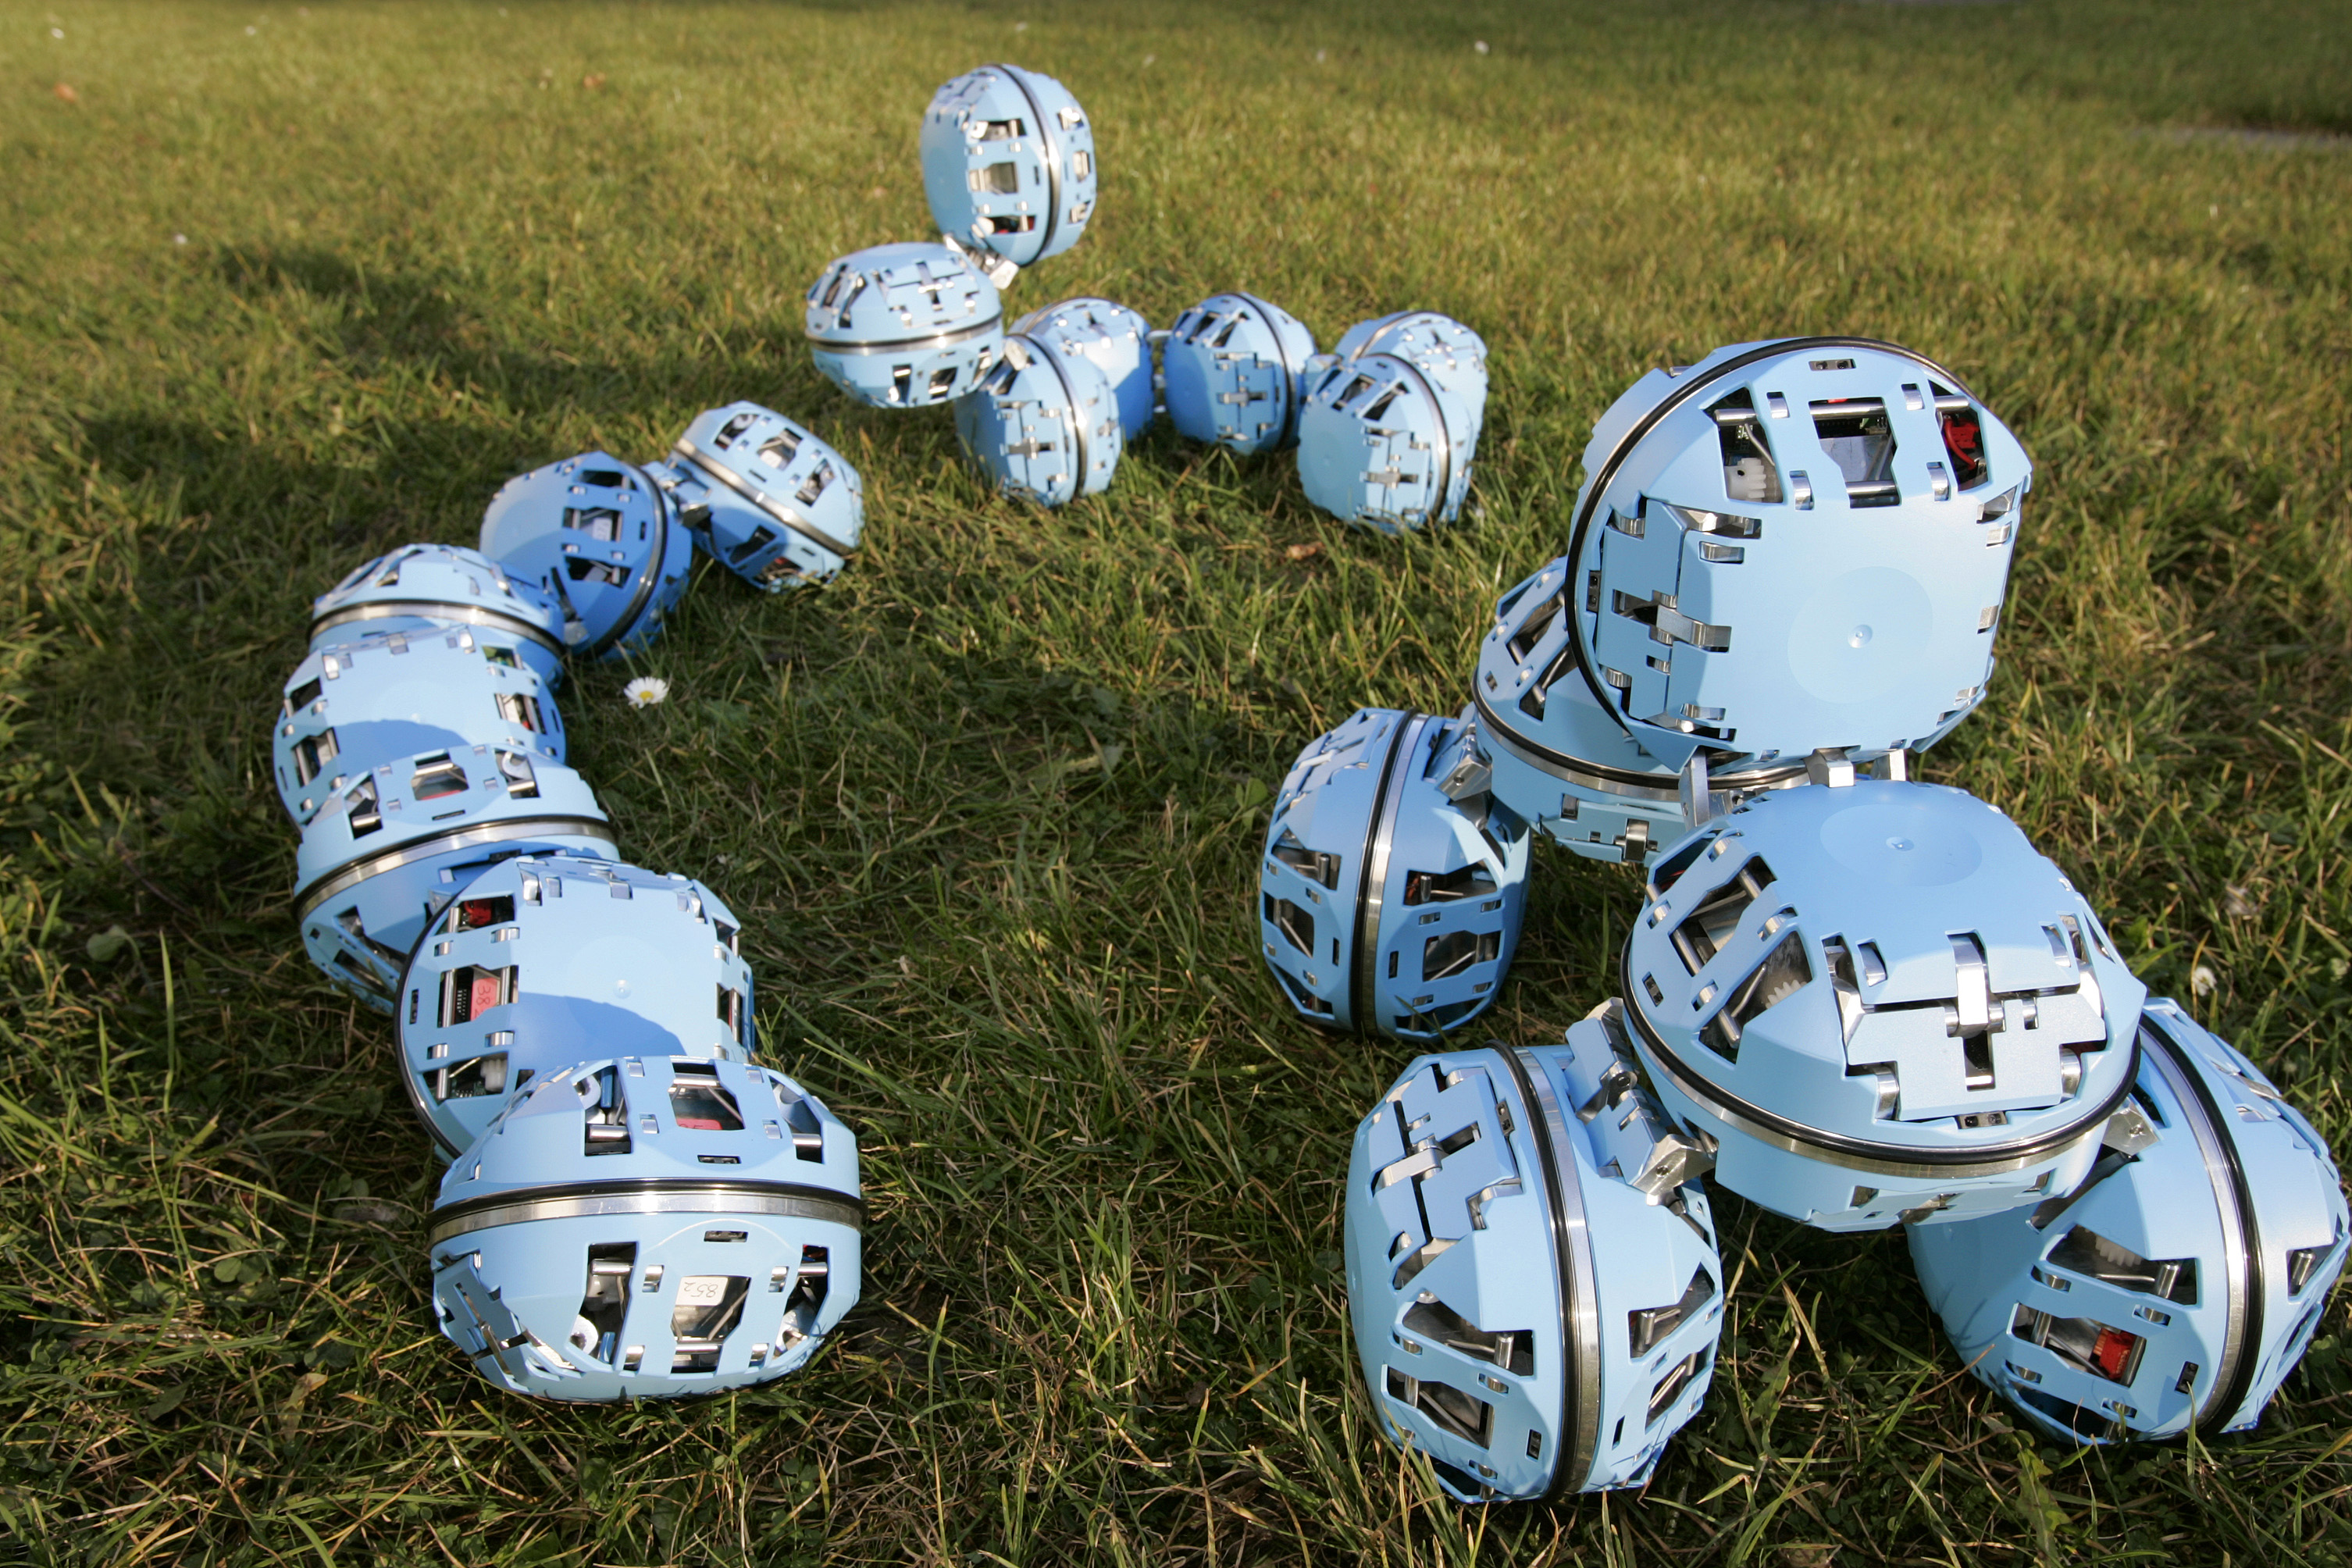
\includegraphics[width=\textwidth]{images/ATRON01.jpg}
                \caption{ATRON}
                \label{fig:ATRON}
        \end{subfigure}
        ~
        \begin{subfigure}[b]{0.18\textwidth}
                \centering
                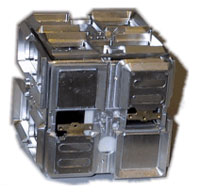
\includegraphics[width=\textwidth]{images/Telecube.jpg}
                \caption{Telecube}
                \label{fig:telecube}
        \end{subfigure}
        ~
        \begin{subfigure}[b]{0.24\textwidth}
         	   \centering
                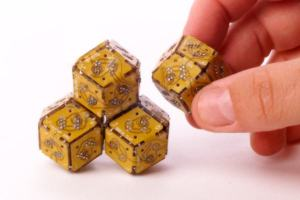
\includegraphics[width=\textwidth]{images/digitalclay.jpg}
                \caption{Digital Clay}
                \label{fig:digital_clay}
        \end{subfigure}        
        ~
        \begin{subfigure}[b]{0.28\textwidth}
         	   \centering
                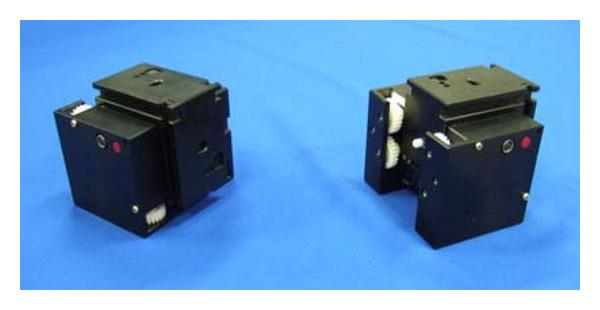
\includegraphics[width=\textwidth]{images/CHOBIE.jpg}
                \caption{CHOBIE}
                \label{fig:chobie}
        \end{subfigure}
        \caption{Examples of lattice-type modular robots}\label{fig:config_lattice_examples}
\end{figure}

In \emph{chain} ( also called \emph{``tree''}) modular robots, the modules are connected forming strings or trees, allowing this kind of robots to reach any point of space. In constrast to this versatility, these modular robots usually need a chain of several modules to reach an arbitrary point, making reconfiguration more complex, and they are more computationally difficult to represent and analyze.\\

Since reconfiguration is more complex in \emph{chain}-type modular robots, they usually achieve locomotion by means of their own bodies or limbs made of modules, performing oscillating patterns with their joints in order to progress towards the goal.\\

Figure \ref{fig:config_chain_examples} contains some examples of chain-type modules, such as CONRO, PolyBot or Y1, on which the modules used in this thesis are based.\\

\begin{figure}[b]
		\centering
        \begin{subfigure}[b]{0.25\textwidth}
                \centering
                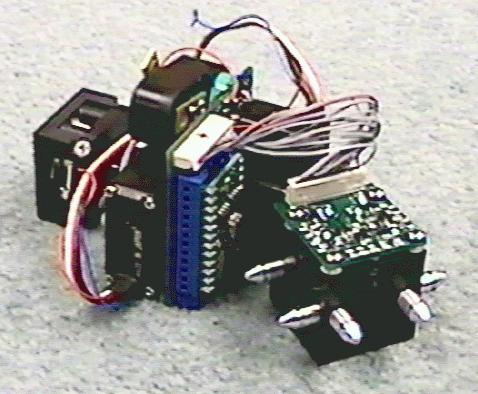
\includegraphics[width=\textwidth]{images/CONRO01.jpg}
                \caption{CONRO}
                \label{fig:CONRO}
        \end{subfigure}
        ~
        \begin{subfigure}[b]{0.18\textwidth}
                \centering
                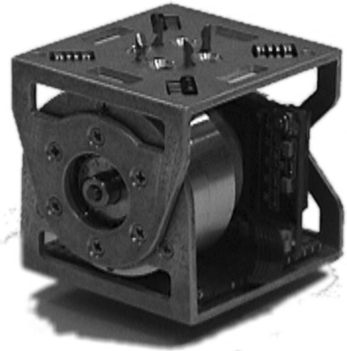
\includegraphics[width=\textwidth]{images/PolyBot_G3.png}
                \caption{PolyBot (G3)}
                \label{fig:PolyBot}
        \end{subfigure}
        ~
        \begin{subfigure}[b]{0.28\textwidth}
         	   \centering
                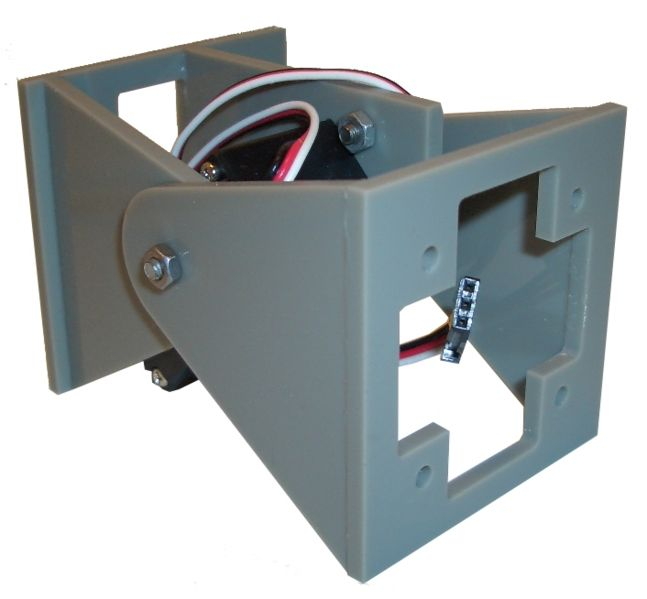
\includegraphics[width=\textwidth]{images/Y1_01.jpg}
                \caption{Y1}
                \label{fig:Y1}
        \end{subfigure}
        \caption{Examples of chain-type modular robots}\label{fig:config_chain_examples}
\end{figure}

The last category of modular robots according to the arrangement of their basic unit are \emph{hybrid} modular robots. These modules have characteristics of both lattice-type and chain-type, allowing them to perform as any of them when required.\\

For reconfiguration the robot behaves as a lattice-type modular robot, since it is easier to model and calculate the steps required for reconfiguration in this type of modules, whereas locomotion is achieved as a chain-type modular robot, obtaining higher speeds and maniobrability this way.\\

Figure \ref{fig:config_hybrid_examples} shows some of the existing \emph{hybrid} modular robots, such as M-TRAN, Superbot or SMORES.\\

\begin{figure}[h]
		\centering
        \begin{subfigure}[b]{0.25\textwidth}
                \centering
                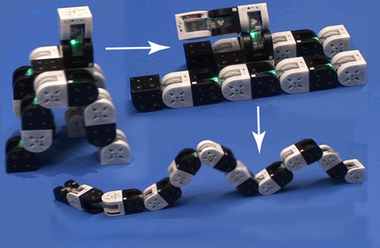
\includegraphics[width=\textwidth]{images/M-TRAN02.jpg}
                \caption{M-TRAN III}
                \label{fig:M-TRAN}
        \end{subfigure}
        ~
        \begin{subfigure}[b]{0.18\textwidth}
                \centering
                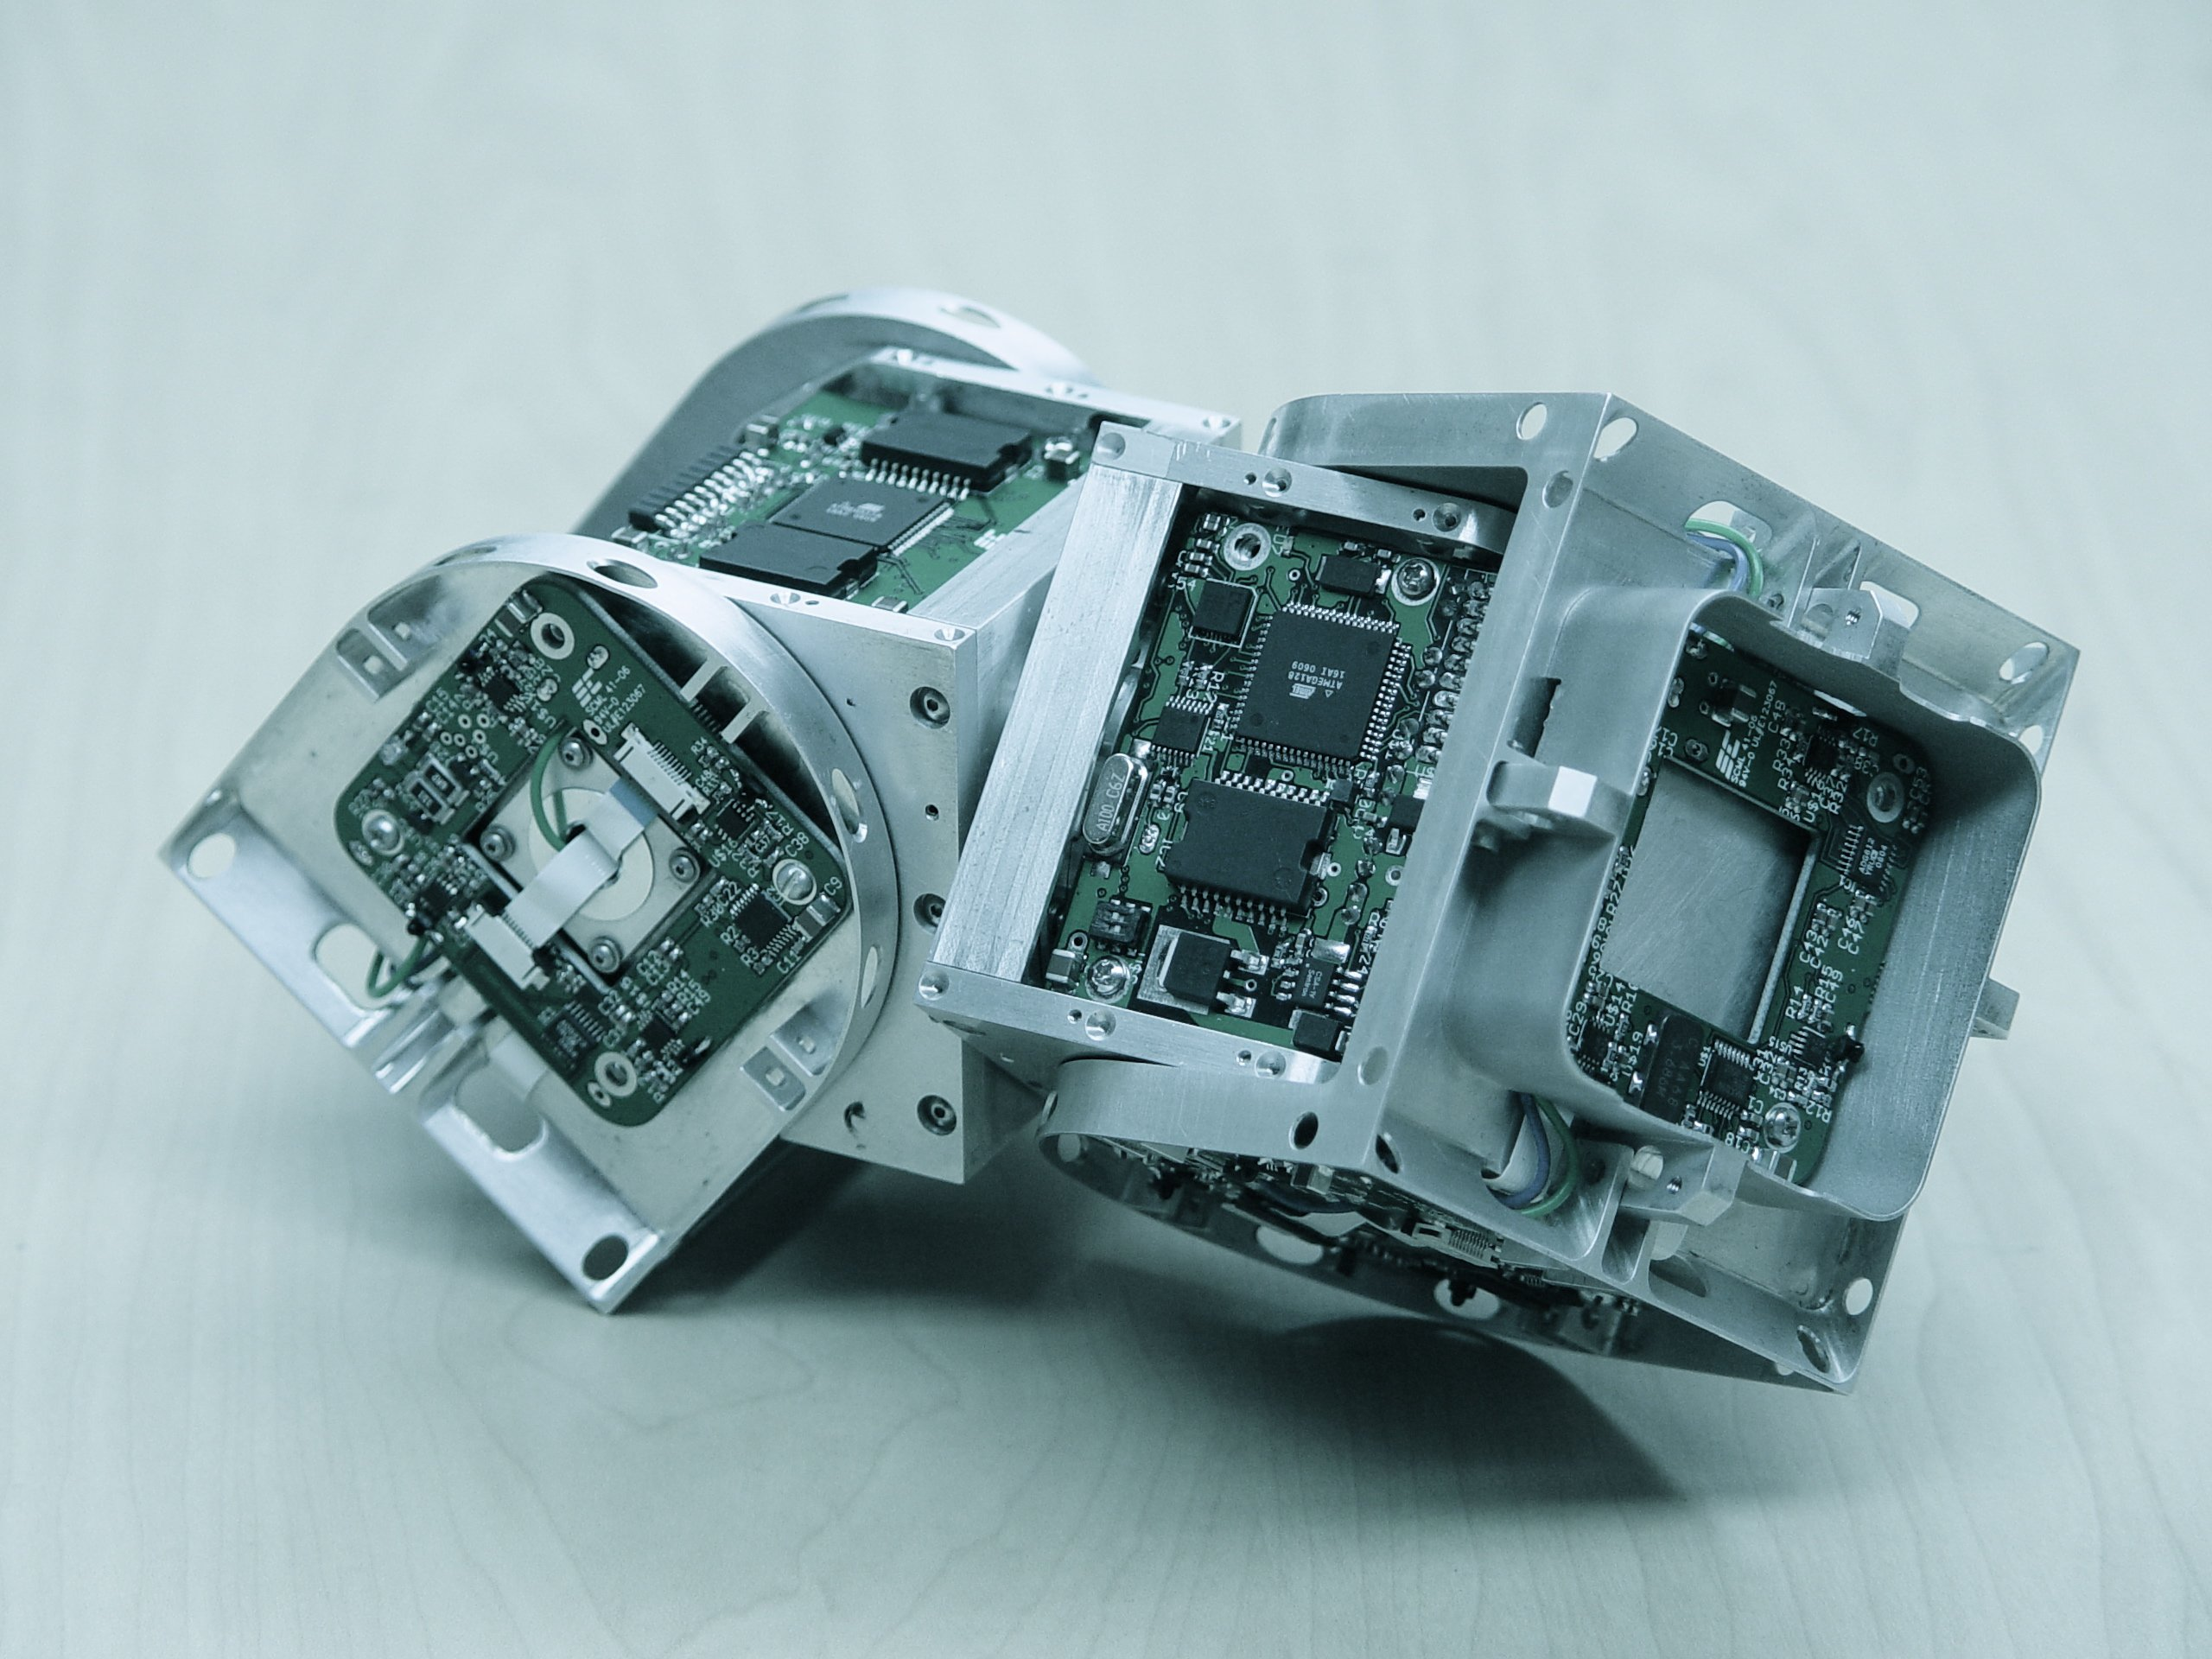
\includegraphics[width=\textwidth]{images/Superbot01.JPG}
                \caption{Superbot}
                \label{fig:Superbot}
        \end{subfigure}
        ~
        \begin{subfigure}[b]{0.28\textwidth}
         	   \centering
                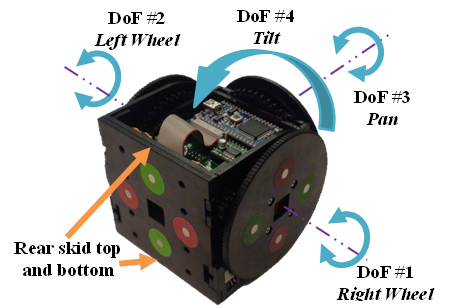
\includegraphics[width=\textwidth]{images/SMORES01.png}
                \caption{SMORES}
                \label{fig:SMORES}
        \end{subfigure}
        \caption{Examples of hybrid-type modular robots}\label{fig:config_hybrid_examples}
\end{figure}



\subsection{Chain-type configurations}
\label{config_chain}

REPY-2.1, the module used in this work, only allows us to build \emph{chain}-type modular robots, and therefore the remaining part of this chapter will focus on them. \emph{Chain}-type modular robots, whose modules form strings or trees, have also several possible configurations, depending on the number of dimensions the trees span (1D, 2D or 3D), that will be addressed in this section.\\

1D chain modular robots resemble snakes or worms and may achieve their gaits with the help of  wheels or tracks, either passive of active (i.e. ``serpentine'' robots), or without them (i.e.  ``snake'' robots), just with their body. The gaits achieved by these configurations can be similar to the side-winding gaits of a snake, to a caterpillar gait or a mix of both, depending on the orientation of their DOFs. They also count with other gaits such as turning or rolling over themselves \cite{}.\\

These 1D configurations are useful for accessing complicated and narrow places, such as holes in the debris or all kinds of pipes. With the suitable gait, these robots can also climb pipes at angles up to 90º though the interior or the exterior of the pipe. One of the most advanced examples of snake robots has been built at the Biorobotics laboratory at the Carnagie Mellon Universy, which can perform all the mentioned gaits, climb trees and even twist around a tree branch when throw onto them \cite{}.\\


Modules that possess connectors on their sides allow 2D configurations. This group of configurations include legged robots (like tripods, quadruped, hexapods, miriapods) and other more exotic mesh-like robots.\\

2D configurations are more complex to describe and model, but they are usually more stable as the count with a larger number of support points over a wider area. {\color{red} Continue this...}\\

2D legged robots can have 1 or more DOF per limb. This thesis is focused on legged robots with multiple DOFs per limb. This kind of configurations require not only coordination among the different limbs (inter-limb coordination) but also coordination among the distinct DOFs inside of each limb (intra-limb coordination) in order to generate a viable gait. They are also more difficult to control, as the longer the limb, the easier from them to collide with other modules in the robot, so the controller has to take into account these contraints when generating the joint values for each module.\\

The last type of chain-type modular robot are 3D configurations. These kind of configurations are very rare, since they are much more complex than 2D configurations, and usually more unstable and harder to reconfigure, which makes them less practical than 2D configurations. One of the few examples from this category are the Roombots, developed by Auke Jan Ijspeert at the École Polytechnique Fédérale de Lausanne (EPFL)\cite{}, whose main goal is to develop adaptative furniture than can adapt to the user needs and reconfigure in whatever piece of furniture that is needed by the user at that moment. Note that the Roombots are hybrid-type modular robots, and for the reconfiguration of the different pieces of furniture the lattice mode is used.\\

Figure \ref{fig:config_chain_examples_extended} shows some examples of the three configurations of chain-type modular robots.\\

\begin{figure}[h]
		\centering
        \begin{subfigure}[b]{0.3\textwidth}
                \centering
                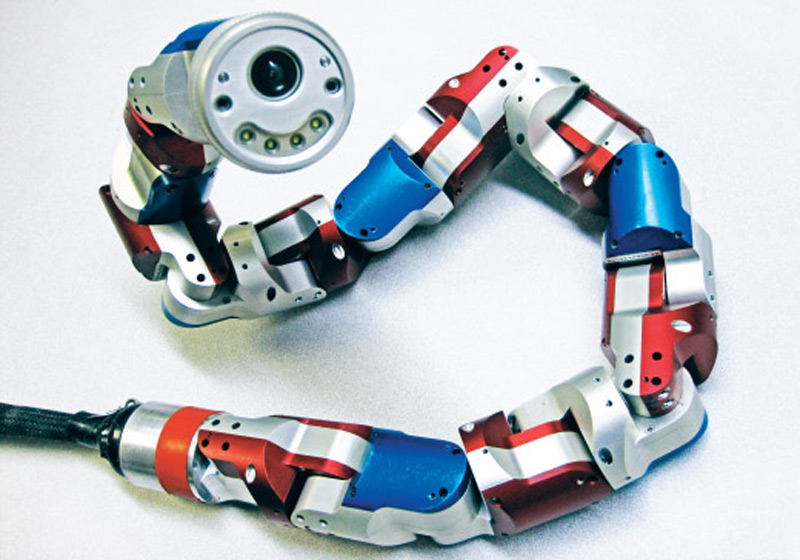
\includegraphics[width=\textwidth]{images/Conf_1D_CMU_snake_robot.jpg}
                \caption{1D: CMU Snake Robot}
                \label{fig:config_1D}
        \end{subfigure}
        ~
        \begin{subfigure}[b]{0.3\textwidth}
                \centering
                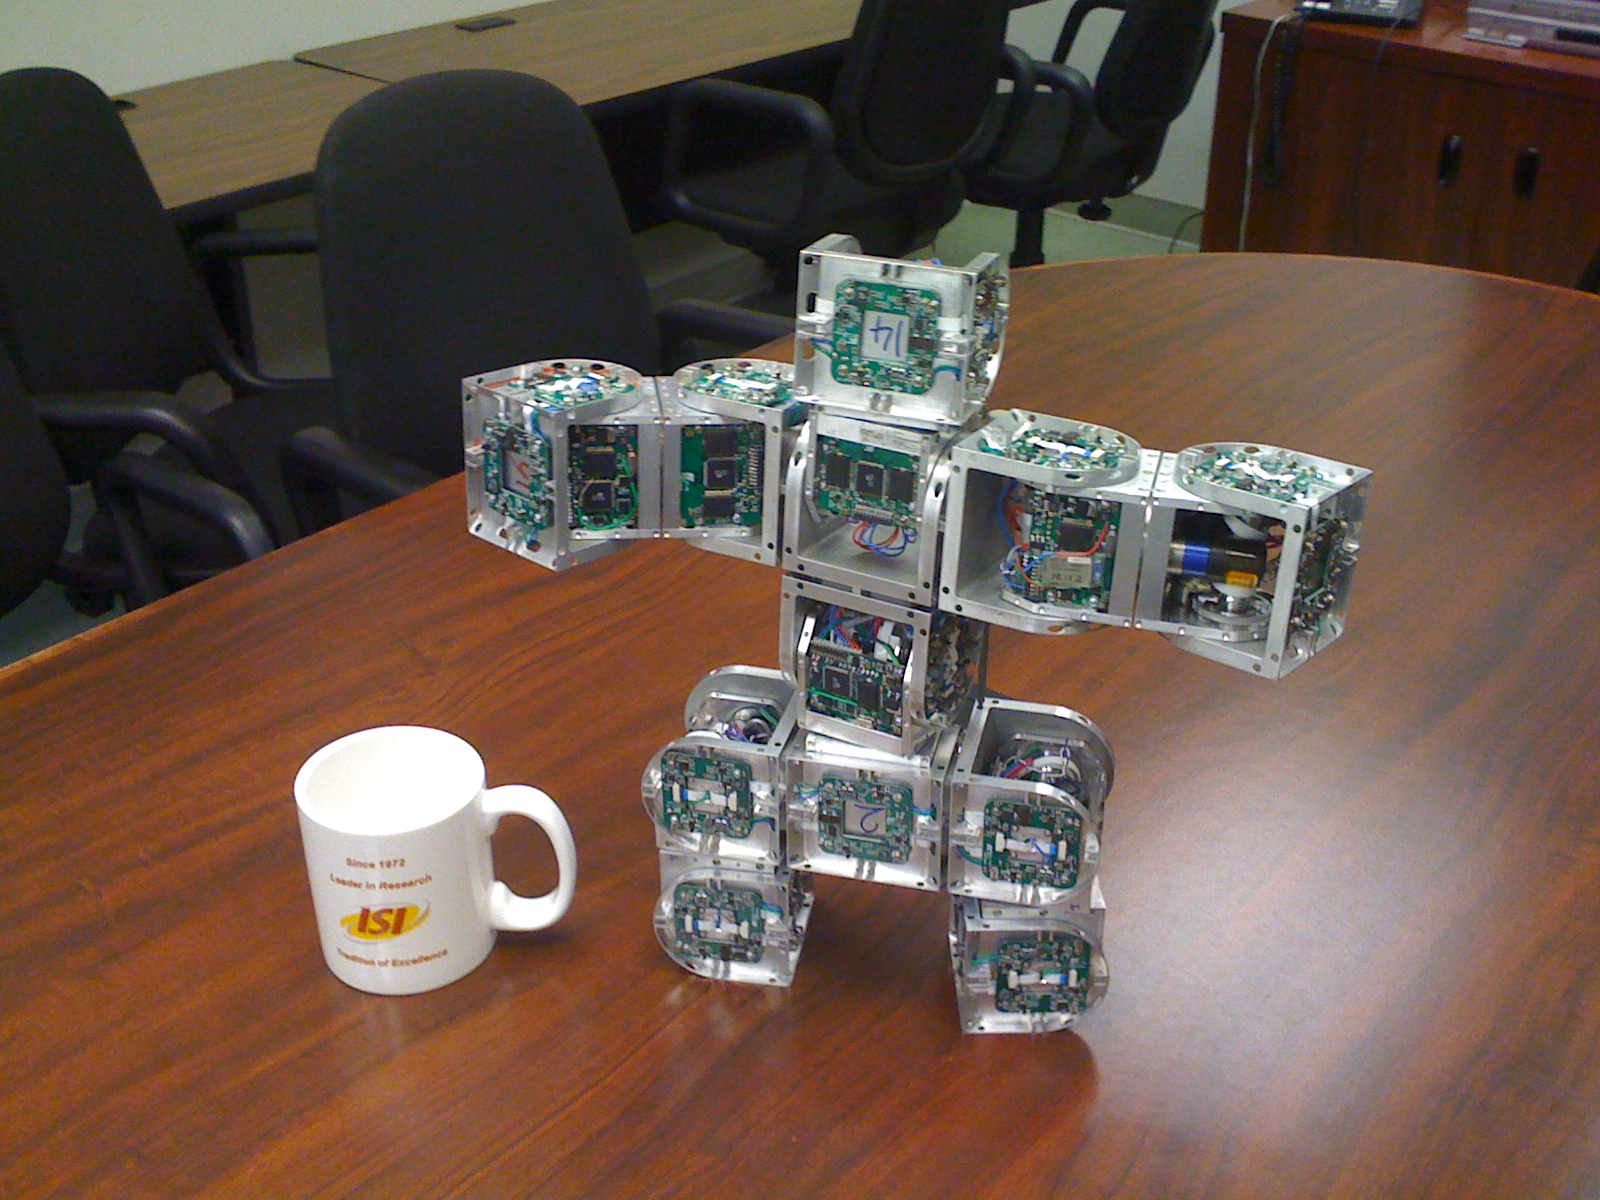
\includegraphics[width=\textwidth]{images/Conf_2D_superbot.jpg}
                \caption{2D: Superbot as mini-humanoid}
                \label{fig:config_2D}
        \end{subfigure}
        ~
        \begin{subfigure}[b]{0.3\textwidth}
         	   \centering
                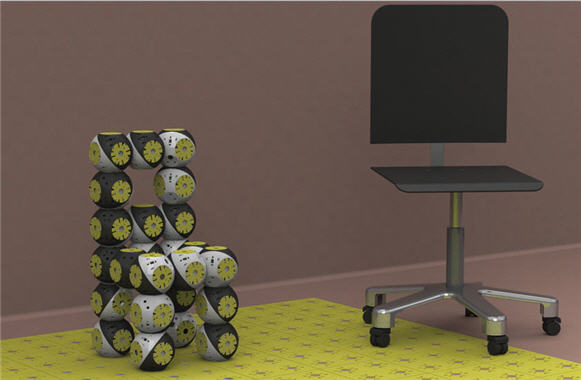
\includegraphics[width=\textwidth]{images/Conf_3D_roombots.jpg}
                \caption{3D: Roombots configured as a chair}
                \label{fig:config_3D}
        \end{subfigure}
        \caption{Examples of the different configuration types of chain modular robots}
        \label{fig:config_chain_examples_extended}
\end{figure}



\subsection{REPY-2.1 available configurations}
\label{config_repy_confs}
The modules used in this thesis are REPY-2.1 modules, a derivative module from the Y1 module designed by Juan Gonzalez-Gomez. REPY-2.1 are very cheap and simple, since they only have 1 DOF controlled by a hobby servo, a 3D printed plastic structure, and the robot is controlled by a central control board, but they lack the features of other more expensive modular robotic platforms, such as self-reconfigurability, indepent in-module control board and autonomy. Despite the lack of those features, these modules are a good platform for researching locomotion gaits for modular robots, since locomotion is achieved in chain-type robots without involving reconfiguration. For the research of the locomotion gaits is enough with the ``skeleton'' of the modular robot, and the REPY-2.1 provides that ``skeleton'' in a cheap and simple way.\\

These modules are interconnected by hand, using screws, and carry a total of 4 connectors, placed in two pairs located in two ortogonal planes. Therefore, REPY-2.1 modules allow both 1D and 2D configurations and, as the module do not possess any means of self-reconfiguring, only chain-type configurations are of interest. They are also genderless and symmetrical, so each pair of connectors can be connected in 4 different positions, with an offset of 90º, yielding a very high number of possible ways of connecting the modules.\\

For the study of the locomotion gaits in legged modular robots with multiple degrees of freedom per limb, three of these configurations are selected. The first of them is a configuration with 2 DOF per limb, 4 limbs, and made of 11 modules, called \emph{``MultiDof-11-2''}, shown in figure \ref{fig:config_repy2_multidof-11-2}.\\

\begin{figure}[b]
		\centering
        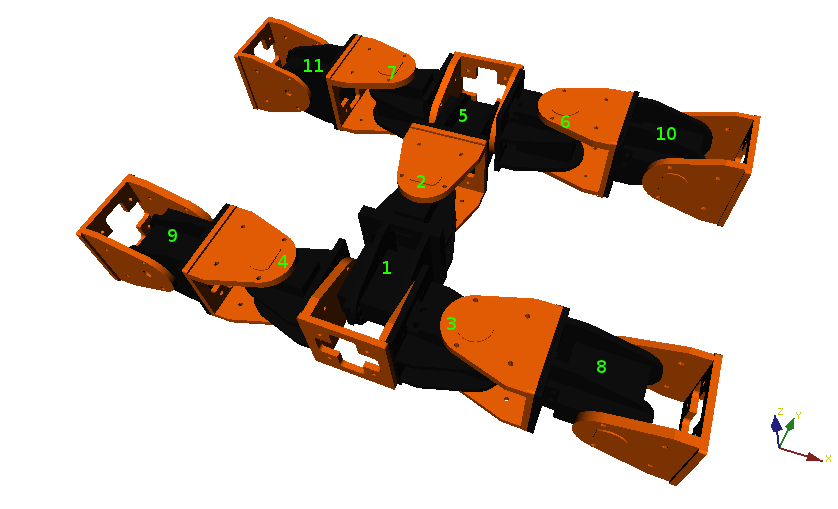
\includegraphics[width=0.5\textwidth]{images/Conf_repy2_multidof-11-2.png}
        \caption{MultiDof-11-2}
        \label{fig:config_repy2_multidof-11-2}
\end{figure}

If we remove the two front limbs (Modules 6, 7, 10 and 11), we obtain a tripod configuration made of 7 REPY-2.1 modules called \emph{``MultiDof-7-tripod''}, and shown in figure \ref{fig:config_repy2_multidof-7-tripod}.\\

\begin{figure}[t]
		\centering
        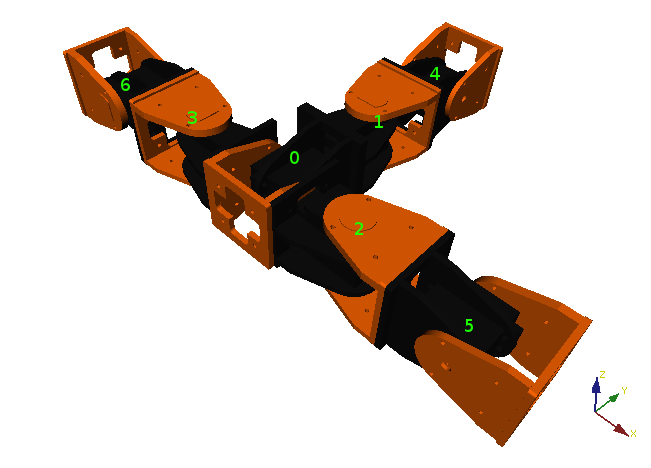
\includegraphics[width=0.5\textwidth]{images/Conf_repy2_multidof-7-tripod.png}
        \caption{MultiDof-7-tripod}
        \label{fig:config_repy2_multidof-7-tripod}
\end{figure}

The last of the configurations is obtained by attaching a fourth leg to the central module of the \emph{``MultiDof-7-tripod''} configuration, obtaining a quadruped configuration made of 9 modules and called \emph{``MultiDof-9-quad''}, that is shown in figure \ref{fig:config_repy2_multidof-9-quad}.\\

\begin{figure}[h]
		\centering
        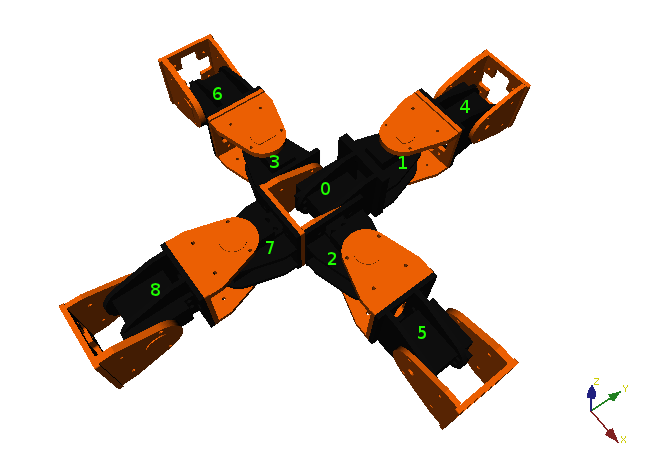
\includegraphics[width=0.5\textwidth]{images/Conf_repy2_multidof-9-quad.png}
        \caption{MultiDof-9-quad}
        \label{fig:config_repy2_multidof-9-quad}
\end{figure}



\subsection{REPY-2.1 configuration description}
\label{config_repy_description}
As described in the previous section, the REPY-2.1 modules can be connected in a large variety of ways {\color{red} (WTF?)}. In order to describe the current location and orientation of a module inside the modular robot, we need to encode all those different ways of connecting the modules, to be able to save the locomotion parameters from a module to the gait table, and later assign those parameters to a module in the same position, that is, performing the same function.\\

The first thing to encode is which of the connectors of the module are being used and which connectors of the neighbor modules are they attached to. Each module has a total of 4 connectors: front, right, back and left, which are encoded in that order to integers from 0 to 3. When two connectors are attached together, as they are symmetrical, they can be connected in four different orientations, each of them obtained from rotating the module to be connected in 90º steps around the vector normal to the connector. Since they can only be connected in steps of 90º, the relative orientation between modules also can be encoded using integers from 0 to 3, representing orientations of 0º, 90º, 180º and 270º.\\

It is possible to calculate the number of possible combinations between modules in an easy way. Let us consider the possible combinations between a single connector of a module and any of the connectors of other module, we have 4 possible connectors to attach to it, and 4 different orientations in which attach them, plus an extra possibility of not having a connector attached to out connector, which yields $4^2+1 = 17$ possibilities. Since we have 4 different connectors in the module, and each connector has 17 possible ways of connecting a module, we have a total of $17^4 = 83521$ combinations.\\

If we were to consider the possible combinations considering also the level 1 neighbors (the neighbors of the neighbors of the considered module), this amount would increase exponentially, and it would be computationally expensive to calculate and store this encoded configurations for each module. That is the reason why in this thesis only level 0 neighbors are considered and, when the ID obtained is ambiguous, some extra info is used to resolve the ambiguities.\\

To encode the different configurations to a number, the following formula is used:
\begin{equation} \label{eq:ID_calculation}
ID = \sum_{i=0}^{3}{ [( x_0^i \cdot 4^0+ x_1^i \cdot 4^1) \cdot x_2^i + 16 \cdot (1-x_2^i)] \cdot 17^i}
\end{equation}

\begin{equation} \label{eq:ID_calculation_extended}
\begin{split}
ID = [( x_0^0 \cdot 4^0+ x_1^0 \cdot 4^1) \cdot x_2^0 + 16 \cdot (1-x_2^0)] \cdot 17^0 + [( x_0^1 \cdot 4^0+ x_1^1 \cdot 4^1) \cdot x_2^1 + 16 \cdot (1-x_2^1)] \cdot 17^1 + \\
 + [( x_0^2 \cdot 4^0+ x_1^2 \cdot 4^1) \cdot x_2^2 + 16 \cdot (1-x_2^2)] \cdot 17^2 + [( x_0^3 \cdot 4^0+ x_1^3 \cdot 4^1) \cdot x_2^3 + 16 \cdot (1-x_2^3)] \cdot 17^3
\end{split}
\end{equation}
~\\
Where:
\begin{itemize}
	\item $i$ is the local connector to be considered, encoded as integer from 0 to 3. 0 corresponds to the \emph{front} connector, 1 to the \emph{right} connector, 2 to the \emph{back} connector and , 3 to the \emph{right} connector.
	\item $x_0^i$ corresponds to the connector of the remote module that is connected, also encoded as integer from 0 to 3. The encoding is identical to the local connector: 0 corresponds to the \emph{front} connector, 1 to the \emph{right} connector, 2 to the \emph{back} connector and , 3 to the \emph{right} connector.
	\item $x_1^i$ corresponds to the relative orientation between the two modules considered, encoded as an integer from 0 to 3. This integer expresses the number of 90º steps around the normal of the connector face required to achieve the given orientation from the default one. A formal description of this parameter is given later on this section.
	\item $x_2^i$ can be either 0 or 1, and represents whether the connector $i$ has a module connected or not. 0 represents ``no module connected'' and 1 that the connector is active.
	\item $4$, $16$ and $17$ are constants representing the number of possibilites of each parameter. Remote connector and orientation are expressed in base 4, since the number of possible values is 4, whereas 17 represents the number of possible combinations of connector and orientation, plus the possibility of not having a module connected. As those combinations go from 0 to 15, 16 is used when there is no module attached.
\end{itemize}

Each pair of connectors can be attached together in 4 different orientations, each of them with a difference of 90º, since the connectors are symmetrical. In order to calculate this orientation, the orientation of the local reference system of each of the modules with respect to an absolute frame is used. This relative orientation is obtained with a Inertial Measurement Unit (IMU) containing an accelerometer, a gyroscope and a magnetic compass, using the Earth's gravity and magnetic field to orientate the sensor with respect to a reference frame fixed on the Earth and returning that orientation expressed in Tait–Bryan angles (Roll, pitch and yaw). These sensors are currently not available in the physical modular robot due to hardware limitations, so the values are set by hand in the configuration file, and later read from it.\\

Two of the three degrees of freedom that the module orientation has are determined by the connectors used to attach the modules, being that the reason why we only need to know one angle to determine the relative orientation of the connectors. This angle is defined as \emph{``the angle we have to rotate the local module around the axis in the same direction as the normal vector of the local connector surface, such as the Z axis of the local reference system of both modules coincide''}. This axis corresponds to the X axis for the side connectors (left and right) and the Y axis for the front and back connectors, as shown in figure \ref{fig:config_sysref}. This method assumes that the configuration in \ref{fig:config_example1} is the default one, and the remaining ones are generated by rotating the remote module by a certain angle.\\


\begin{figure}[h]
		\centering
        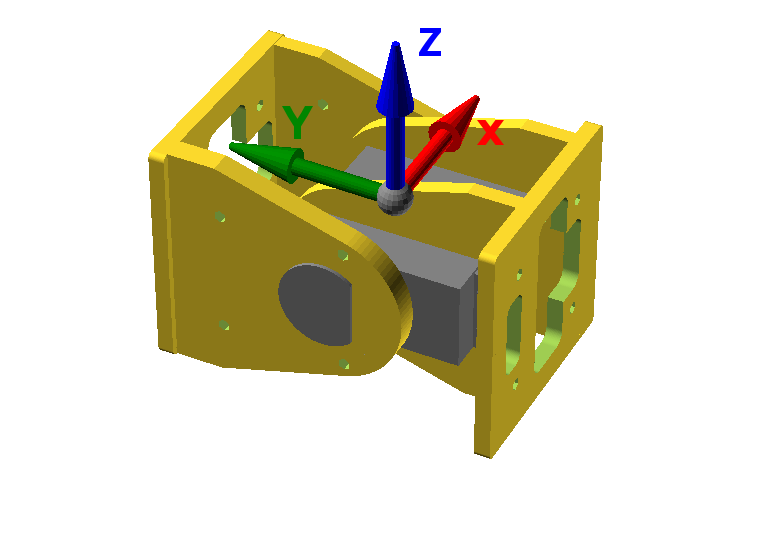
\includegraphics[width=0.4\textwidth]{images/Conf_sysref_module.png}
        \caption{Reference system for REPY-2.1 modules}
        \label{fig:config_sysref}
\end{figure}

Figure \ref{fig:config_example1-4} represents the 4 possible orientations of a simple 2-module configuration with their corresponding orientation value for each of them. If we are calculating the orientation from the rightmost module point of view, we observe that the remote module is connected to the front connector of the local module, and therefore the Y axis of the local module the axis of reference. Around this axis, the local module is turn in 90º steps until both Z axis are coincident. The number of steps required is the value of the orientation parameter.\\

\begin{figure}[h]
		\centering
        \begin{subfigure}[b]{0.35\textwidth}
                \centering
                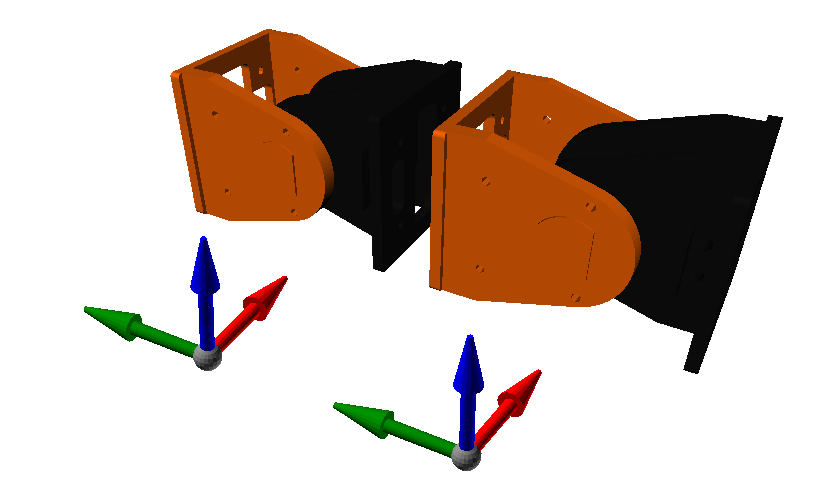
\includegraphics[width=\textwidth]{images/Conf_example_01.png}
                \caption{Aligned modules (orientation value = 0)}
                \label{fig:config_example1}
        \end{subfigure}
        ~
        \begin{subfigure}[b]{0.35\textwidth}
                \centering
                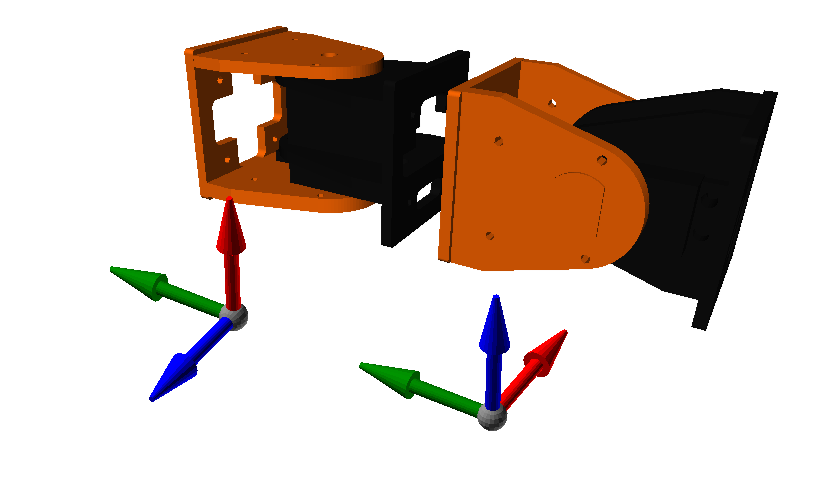
\includegraphics[width=\textwidth]{images/Conf_example_04.png}
                \caption{90º offset (orientation value = 1)}
                \label{fig:config_example2}
        \end{subfigure}
        ~
        \begin{subfigure}[b]{0.35\textwidth}
         	   \centering
                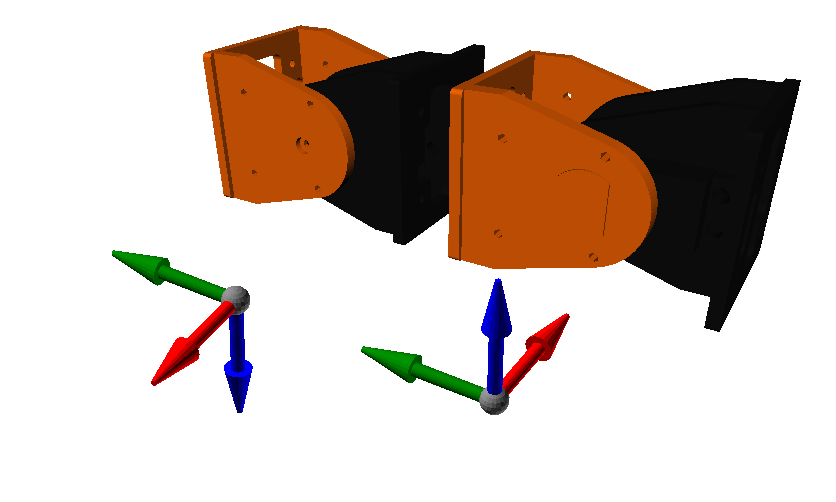
\includegraphics[width=\textwidth]{images/Conf_example_03.png}
                \caption{180º offset (orientation value = 2)}
                \label{fig:config_example3}
        \end{subfigure}
                ~
        \begin{subfigure}[b]{0.35\textwidth}
         	   \centering
                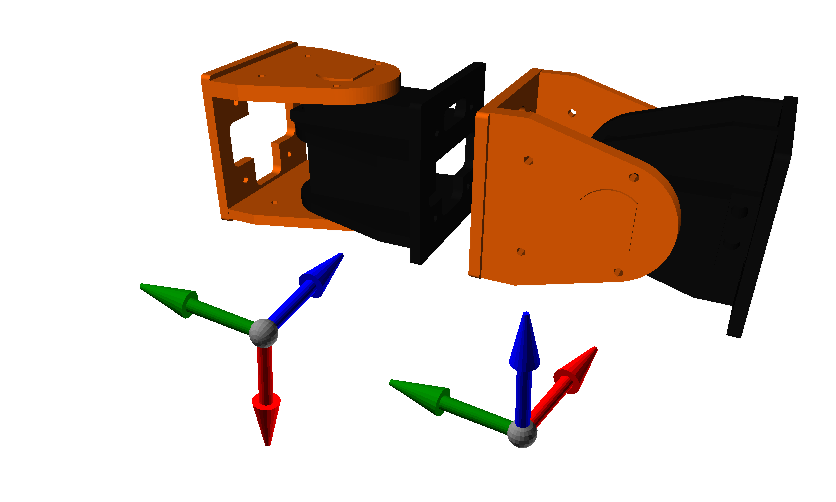
\includegraphics[width=\textwidth]{images/Conf_example_02.png}
                \caption{270º offset (orientation value = 3)}
                \label{fig:config_example4}
        \end{subfigure}
        \caption{Examples of relative orientation on a 2-module configuration}\label{fig:config_example1-4}
\end{figure}
Let us calculate the ID of the third configuration in figure \ref{fig:config_example1-4}, configuration \emph{c}, using equation \ref{eq:ID_calculation}:
\[ID = \sum_{i=0}^{3}{ [( x_0^i \cdot 4^0+ x_1^i \cdot 4^1) \cdot x_2^i + 16 \cdot (1-x_2^i)] \cdot 17^i}\]

Only the front connector is active, so $x_2^i$ equals 0 for connectors 1, 2 and 3. As the front connector is connected to the back connector (encoded as `2') and their relative angle is 180º (encoded also as `2'), the ID would be:
\[ID = ( 2 \cdot 4^0+ 2 \cdot 4^1) \cdot 17^0 +
  16 \cdot 17^1 + 16 \cdot 17^2 + 16  \cdot 17^3 = 83514\]\\
  

Figure \ref{fig:config_example5-8} shows another 2-module configuration, but this time the module is attached to the left connector using its back connector. In this case the reference axis is the X axis of the local module, and is important to notice that the axis of rotation is located in the direction of the local refence system, not in the direction of the connector normal vector. By rotating the remote module in steps of 90º, the 4 possible configurations are generated.\\

\begin{figure}[h]
		\centering
        \begin{subfigure}[b]{0.35\textwidth}
                \centering
                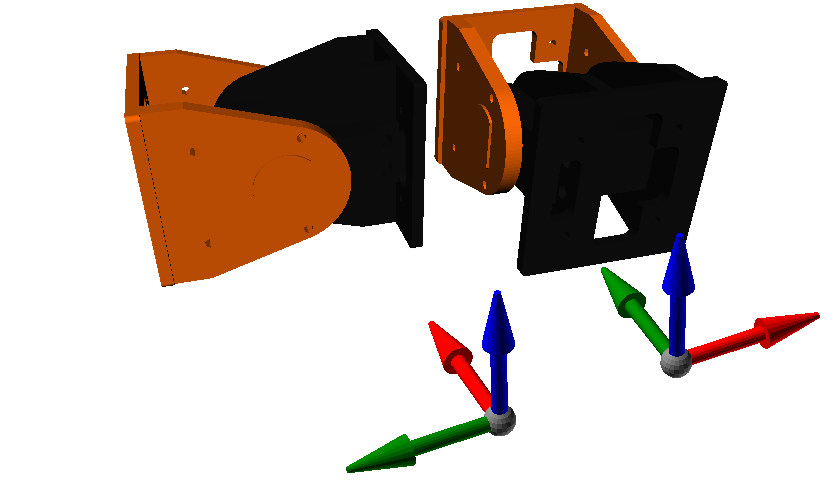
\includegraphics[width=\textwidth]{images/Conf_example_08.png}
                \caption{Aligned modules (orientation value = 0)}
                \label{fig:config_example5}
        \end{subfigure}
        ~
        \begin{subfigure}[b]{0.35\textwidth}
                \centering
                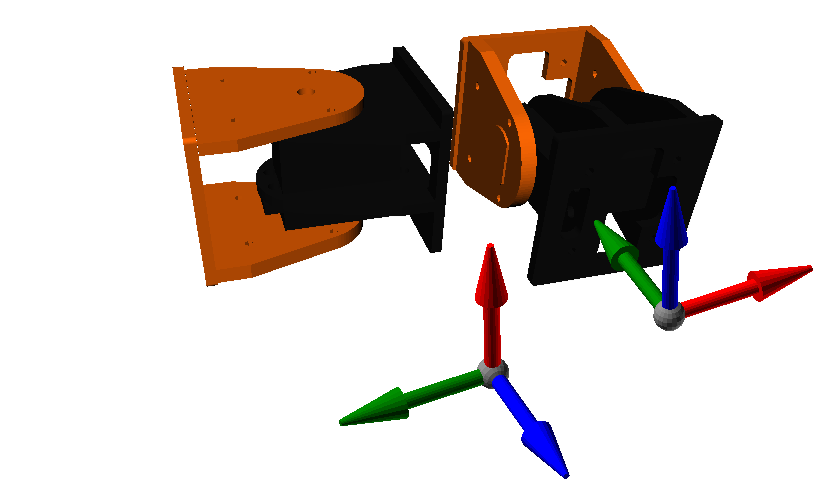
\includegraphics[width=\textwidth]{images/Conf_example_07.png}
                \caption{90º offset (orientation value = 1)}
                \label{fig:config_example6}
        \end{subfigure}
        ~
        \begin{subfigure}[b]{0.35\textwidth}
         	   \centering
                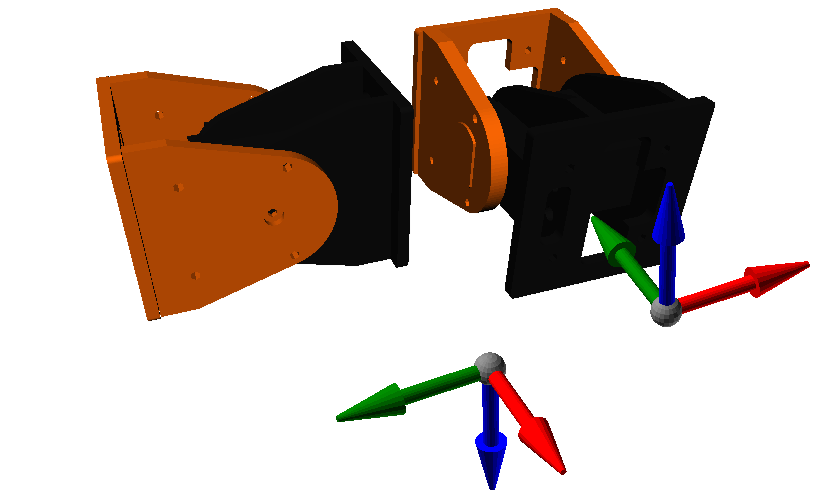
\includegraphics[width=\textwidth]{images/Conf_example_06.png}
                \caption{180º offset (orientation value = 2)}
                \label{fig:config_example7}
        \end{subfigure}
                ~
        \begin{subfigure}[b]{0.35\textwidth}
         	   \centering
                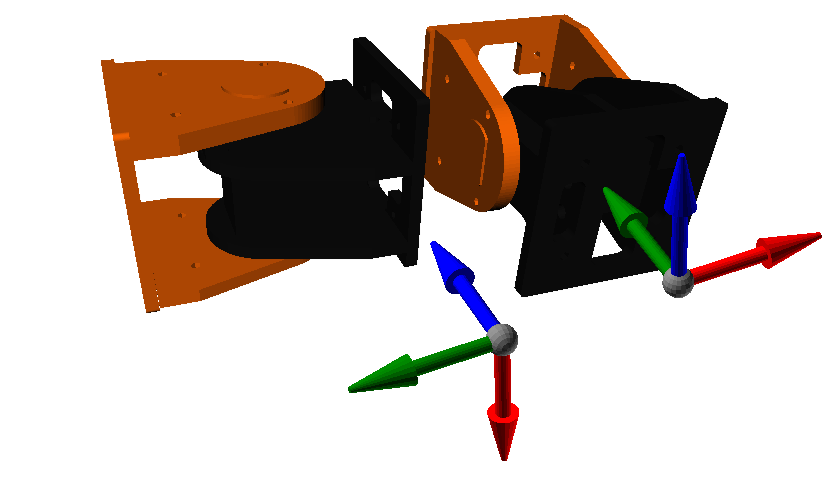
\includegraphics[width=\textwidth]{images/Conf_example_05.png}
                \caption{270º offset (orientation value = 3)}
                \label{fig:config_example8}
        \end{subfigure}
        \caption{Examples of relative orientation on a 2-module configuration}\label{fig:config_example5-8}
\end{figure}

To calculate the ID of the last configuration in figure \ref{fig:config_example5-8}, configuration \emph{d}, we apply again equation \ref{eq:ID_calculation}. In this case, the active connector is the left connector, making $x_2^i=0$ for connectors 0, 1 and 2. If we substitute the remote connector (back connector,`2') and the relative orientation ( 270º, encoded as 3) it yields an ID of:
\[ID =16 \cdot 17^0 + 16 \cdot 17^1 + 16 \cdot 17^2 + ( 2 \cdot 4^0+ 3 \cdot 4^1)  \cdot 17^3 = 73694\]\\

Finally, in figure \ref{fig:config_example9} we can observe a 4 module configuration in which the central module has 3 active connections. For finding the relative orientation of the side connectors, the X axis is used, obtaining a orientation of 270º for the module attached to the right connector and a orientation of 90º for the module attached to the left connector, enconding them as 3 and 1, respectively (the central module is upside-down, so the left hand module in the figure corresponds to the right connector of the central module). For the back connector module, the local Y axis is used, obtaining a relative orientation of 90º, encoded as 1.\\

If we substitute these values in equation \ref{eq:ID_calculation}, we can calculate the ID for the central module:
\[ID =16 \cdot 17^0 +
 ( 2 \cdot 4^0+ 1 \cdot 4^1) \cdot 17^1 +
 ( 2 \cdot 4^0+ 1 \cdot 4^1) \cdot 17^2 +
 ( 2 \cdot 4^0+ 3 \cdot 4^1)  \cdot 17^3 = 31466\]\\
  
\begin{figure}[h]
		\centering
        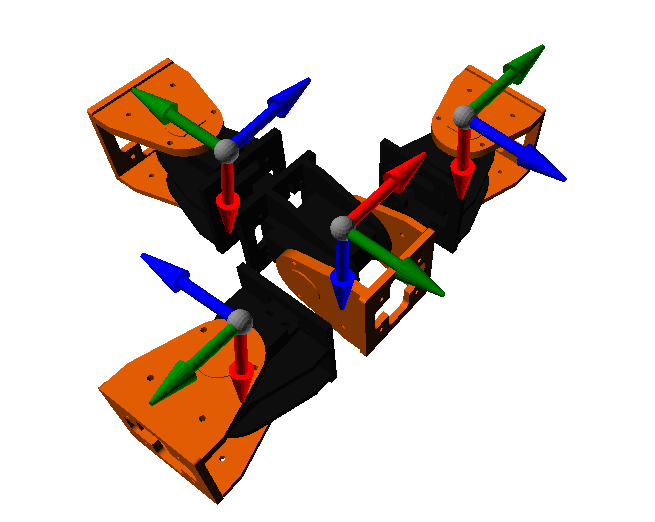
\includegraphics[width=0.5\textwidth]{images/Conf_example_09-01.png}
        \caption{Configuration with 4 modules}\label{fig:config_example9}
\end{figure}

\section{Gait generation}
\label{gaits}

The lower level control for locomotion in mobile robots with wheels or tracks is usually not complicated, since it only involves turning the motors in order to produce movement. Difficulties appear at the higher level control, such as motion planning or navigation.\\

But, when the robot is articulated, either with legs or apodal, the lower level control becomes more complicated, as the problem of coordination appears, even if the robot is to travel through a flat surface without any kind of obstacles. In this kind of robots the movement of each of the joints must be coordinated with the movement of the other joints so that the robot can move. In more formal terms, the coordination problem can be stated as follows: \emph{For a robot with N articulations, find the value of each joint as a function of time $\varphi_i(t)$ so that the robot can achieve locomotion}. The solution of this problem is not unique, and depends on the type of gait that one desires to obtain (e.g. walking on a straight line, turning, trotting, galloping, etc).\\

In order to solve this problem, several approaches can be followed, and they will be explained in this section.\\

\subsection{Gait tables}
\label{gait_gaittables}

Gait tables are tables that include the DOF values for each module at different steps of a gait. For each moment of the gait, each of the modules look up in the table what is the required joint value for the current step, and move their DOFs to that value. When the robot arrives at the end of the table, it starts again with the first position of the table, achieving a repeating pattern.\\

This is an easy and simple way to implement locomotion gaits for modular robots, and was first used by Mark Yim in his PolyPod \cite{}. When the robots are composed of few modules and the desired movements are simple, these gait tables can be formed by hand, allowing a fast exploration of possible gaits for locomotion, as well as detecting mechanical defects on robot prototypes. Gait tables are not only useful for designing gaits for modular robots, but they can also be applied to other types of robots, such as quadruped, hexapods or even humanoid robots.\\

The main disadvantage of gait tables is that they lack flexibility, as for generating new gaits, or variations of the existing gaits, a new control table has to be created.\\

\subsection{Central Pattern Generators (GPGs)}
\label{gait_cpgs}
Central pattern generators (CPGs) are biological neural networks capable of producing coordinated patterns of rhythmic activity without any rhythmic inputs from sensory feedback or from higher control centers \cite{}. They are in charge of many rhythmic behaviours in both vertebrate and invertebrate animals, such as breathing, locomotion, bowel movements, etc.\\

CPGs are distributed networks composed by multiple coupled oscillatory centers, as observed in experiments with lampreys and salamanders, in which small sections of their spinal cords were capable of producing rhythmics activity. The lamprey is one the vertebrates most used to study CPGs, because its spinal column is transparent, contains few cells, and lasts at least a week outside
of the animal (in a saline solution) without deterioration \cite{}, easing the work of the biologists.\\

Sensory feedback is not needed for the generation of the rhythms, but plays a key role in shaping the rhythmic patterns and keeping the body movements and the CPG coordinated. This coupling is so tight that is posible to induce CPG activity mecanically moving the tail of a lamprey, and to induce a normally looking walking gait in a decerebrated \footnote{Decerebration is the elimination of cerebral brain function in an animal by removing the cerebrum, cutting across the brain stem, or severing certain arteries in the brain stem \cite{}.} cat by placing it on a treadmill. If the treadmill is accelerated, the gait can even change from trot to gallop.\\

The complex locomotion behaviour generated by the CPG circuits is controlled by simple signals, that in many vertebrates are generated in a specific region of the brain stem known as \emph{Mesencephalic Locomotion Region} (MLR). Some experiments with electrical stimulation of this region have shown that the level of stimulation can modulate the speed of locomotions, and induce an automatic gait transition (from walk to trot to gallop on derebrated cats, and from walk to swimming on decerebrated salamanders). Therefore, basic rhythmic patters are generated at the spinal CPGs, but the modulation of those patterns according to environmental factors is controlled by the higher-level centers, such as the motor cortex, cerebellum and basal ganglia.\\

These biological CPGs have been matematically modelled as differential equations, and successfully applied to different robots, such as the Salamandra Robotica, a salamander-like robot developed at the EPFL \cite{}. Since CPGs are a distributed approach, it has been also applied to modular robots, such as YaMoR \cite{} or the Roombots \cite{}. One advantage of using CPGs is that the transitions between two steady state oscillations is bounded, continuous and relatively smooth, so if we are implementing an optimization algorithm for the gaits, and we randomly change the control parameters, the joint values will not change too abruptly, which helps preventing the motors from breaking \cite{}.\\

\subsection{Sinusoidal Oscillators}
\label{gait_sin_osc}

CPGs are very powerful controllers, but they are also very complex to model and implement, and highly redundant. These CPG mathematical models are useful for neurocomputing scientists to study biological CPGs and model neural circuits, as they can be tested either on simulations or on real robots, and therefore validated. In robotics, on the other hand, one is often more interesting in efficiency, in obtaining the best possible gaits using as less resources, computing power and power as possible.\\

In order to achieve this, we can substitute the CPG model obtained by neurocomputing scientis by a simpler one that performs in a similar way, but using less resources. CPGs behave as fixed frequency oscillators in steady state, making sinusoidal oscillator a suitable canditate for being used as gait generators, as they are much simpler to model and require less resources for their implementation than CPGs.\\

These sinusoidal oscillators are modeled by the following equation:
\begin{equation} \label{eq:sinusoidal_oscillator}
\varphi_i(t) = A_i \cdot \sin{\left( \frac{2\pi}{T} \cdot t + \Phi_i \right)} + O_i \qquad i \in \lbrace 1, ..., N \rbrace 1
\end{equation}


\begin{table}[h]
\centering
\begin{tabular}{|c||c|c|} \hline
Symbol & Description & Range \\ \hline \hline
$\varphi_i(t)$ & Position of the ith joint & [-90, 90] degrees \\ \hline
$A_i$ & Amplitude of the ith oscillator & [0, 90] degrees \\ \hline
$T$ & Period of the oscillator &  T > 0 seconds \\ \hline
$t$ & Elapsed time & t $\leq$ 0 seconds \\ \hline
$\Phi_i$ & Initial phase of ith oscillator & [0, 360] degrees \\ \hline
$O_i$ & Offset of ith oscillator & [-90, 90] degrees \\ \hline
$N$ & Number of modules in the robot & $N \geq 2$ \\ \hline
\end{tabular}
\caption{Parameters of the sinusoidal oscillator}
\end{table}

The frequency of the oscillators does not affect the coordination, but the speed of the gait. The main parameter behind gait coordination is the phase of the oscillator, defined as:

\begin{equation} \label{eq:phase_of_time}
\phi(t) = \frac{2\pi}{T} \cdot t
\end{equation}\\

Which can be substituted in equation \ref{eq:sinusoidal_oscillator} to get the joint value of the ith oscillator as a function of the phase:

\begin{equation} \label{eq:sinusoidal_oscillator_phase}
\varphi_i(\phi) = A_i \cdot \sin{\left( \phi + \Phi_i \right)} + O_i \qquad i \in \lbrace 1, ..., N \rbrace 1
\end{equation}\\

As the modules are physically actuated by a hobby servo, with a mechanical restriction of 180 degrees, we have limited the oscillator joint values to  a range of [-90, 90] degrees, imposing the following restriction to the oscillator parameters:
\begin{equation} \label{eq:oscillator_restriction}
|O_i| + A_i \leq 90
\end{equation}

Figure \ref{fig:oscillator_center_seq} helps to understand the physical meaning of the equation parameters. In this case, the amplitude is 45º and the offset is 0º, so the movement is centered around the 0º joint position. The minimum position reached by the joint is $ O - A = -45º$ and the maximum one is $O + A = 45º$, following a sinusoidal waveform as a function of time.\\

\begin{figure}[h]
		\centering
        \begin{subfigure}[b]{0.18\textwidth}
                \centering
                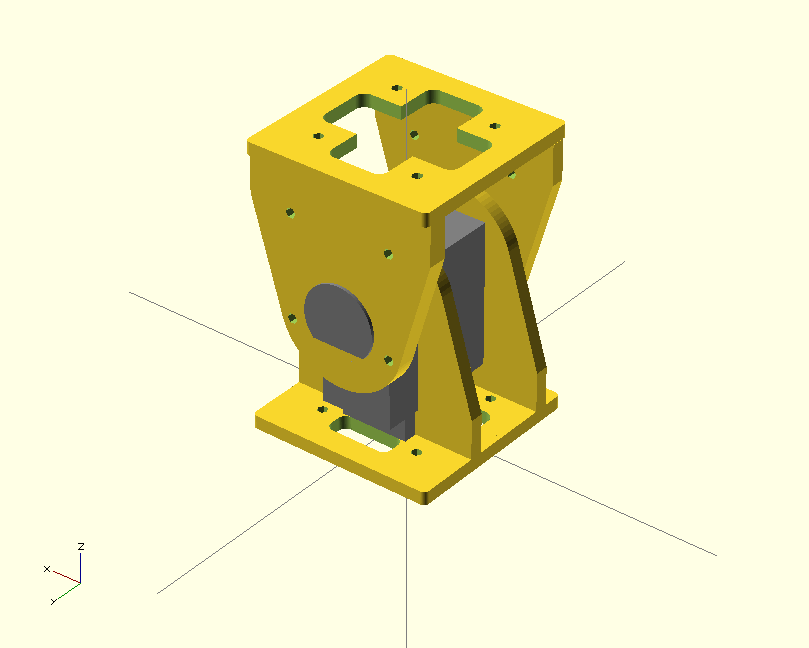
\includegraphics[width=\textwidth]{images/Gait_osc_center_90.png}
                \caption{$t = 0$, $\phi=0º$}
                \label{fig:Gait_osc_center_90}
        \end{subfigure}
        ~
        \begin{subfigure}[b]{0.18\textwidth}
                \centering
                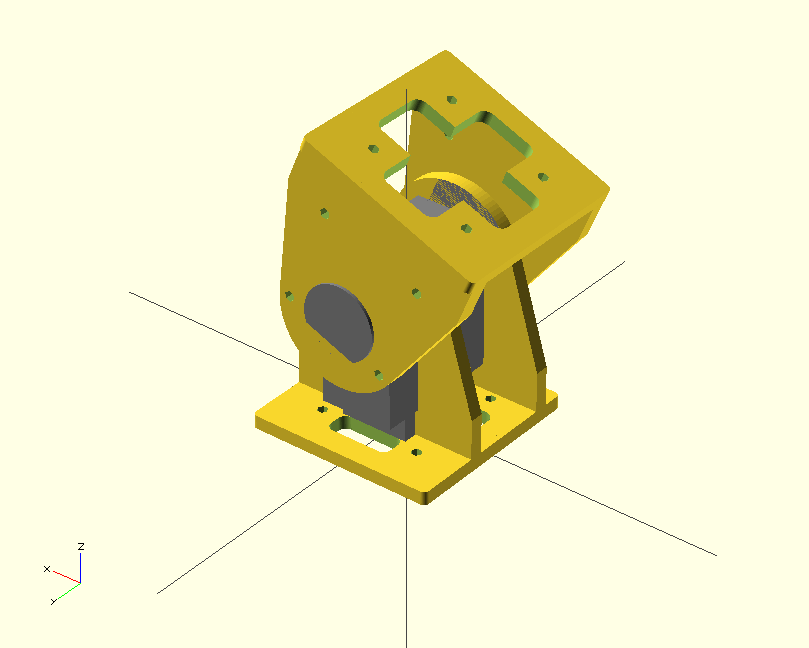
\includegraphics[width=\textwidth]{images/Gait_osc_center_112_5.png}
                \caption{$t = $, $\phi=º$}
                \label{fig:Gait_osc_center_112_5}
        \end{subfigure}
        ~
        \begin{subfigure}[b]{0.18\textwidth}
         	   \centering
                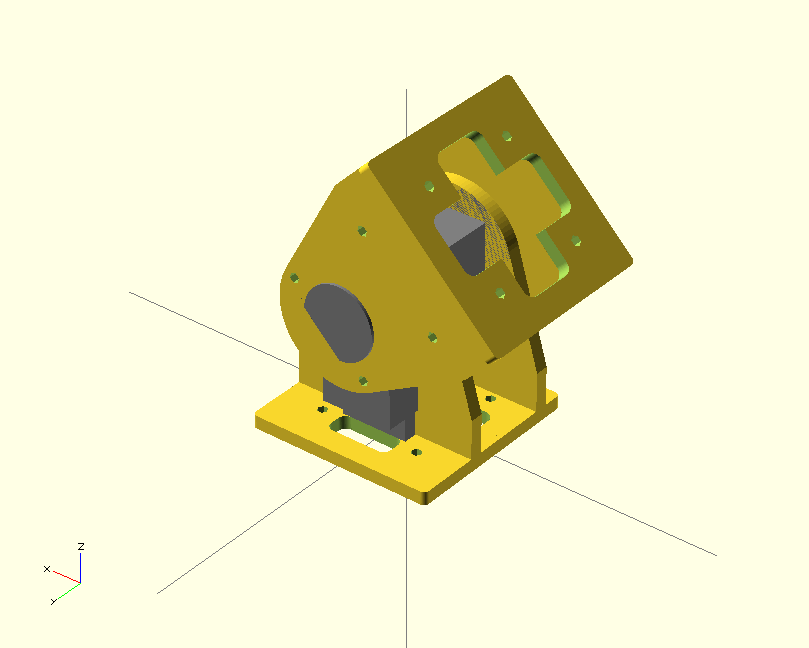
\includegraphics[width=\textwidth]{images/Gait_osc_center_135.png}
                \caption{$t = \frac{T}{4}$, $\phi=90º$}
                \label{fig:Gait_osc_center_135}
        \end{subfigure}
        ~
        \begin{subfigure}[b]{0.18\textwidth}
         	   \centering
                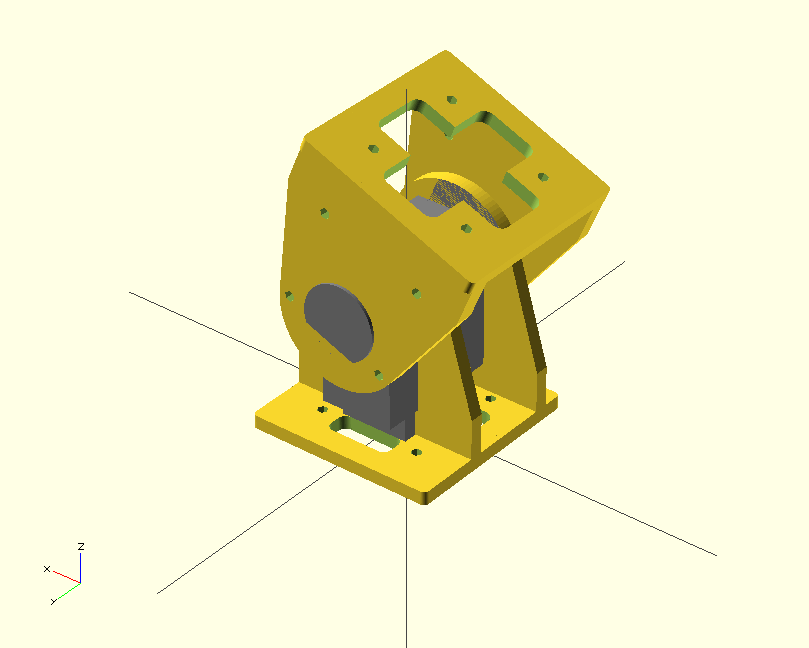
\includegraphics[width=\textwidth]{images/Gait_osc_center_112_5.png}
                \caption{$t = $, $\phi=º$}
                \label{fig:Gait_osc_center_112_5-2}
        \end{subfigure}
        ~
        \begin{subfigure}[b]{0.18\textwidth}
         	   \centering
                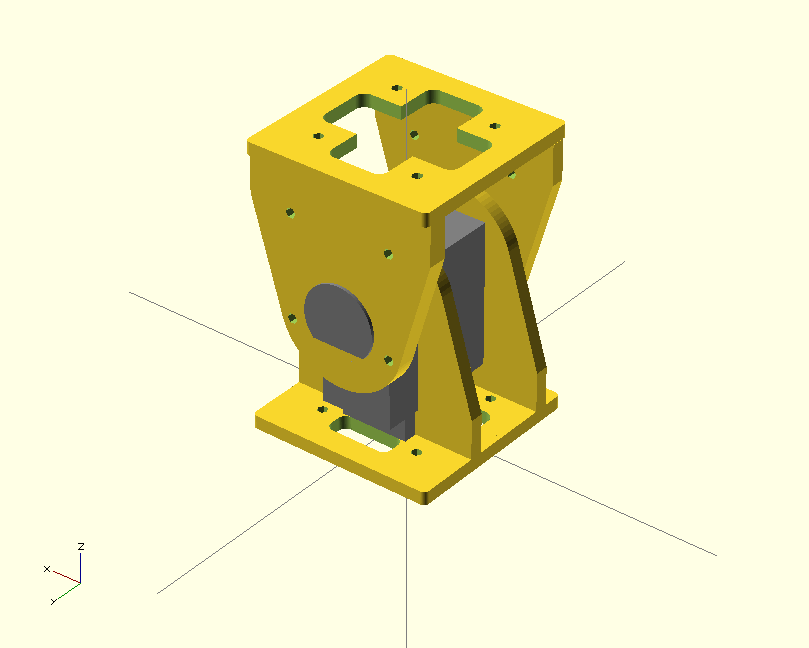
\includegraphics[width=\textwidth]{images/Gait_osc_center_90.png}
                \caption{$t = \frac{T}{2}$, , $\phi=180º$}
                \label{fig:Gait_osc_center_90-2}
        \end{subfigure}
        ~
                \begin{subfigure}[b]{0.18\textwidth}
                \centering
                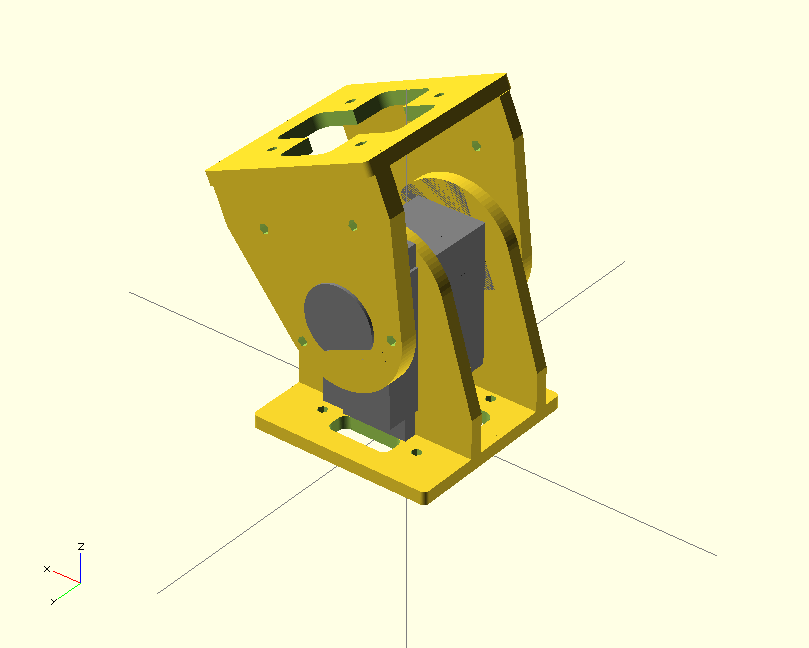
\includegraphics[width=\textwidth]{images/Gait_osc_center_62_5.png}
                \caption{$t = $, $\phi=º$}
                \label{fig:Gait_osc_center_62_5-2}
        \end{subfigure}
        ~
        \begin{subfigure}[b]{0.18\textwidth}
                \centering
                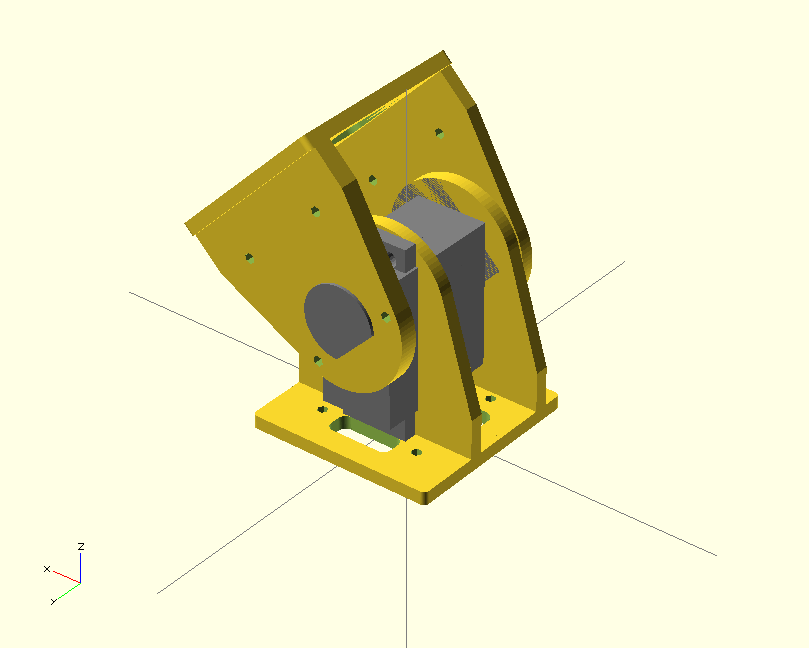
\includegraphics[width=\textwidth]{images/Gait_osc_center_45.png}
                \caption{$t = \frac{3T}{4}$, $\phi=270º$}
                \label{fig:Gait_osc_center_45-2}
        \end{subfigure}
        ~
        \begin{subfigure}[b]{0.18\textwidth}
         	   \centering
                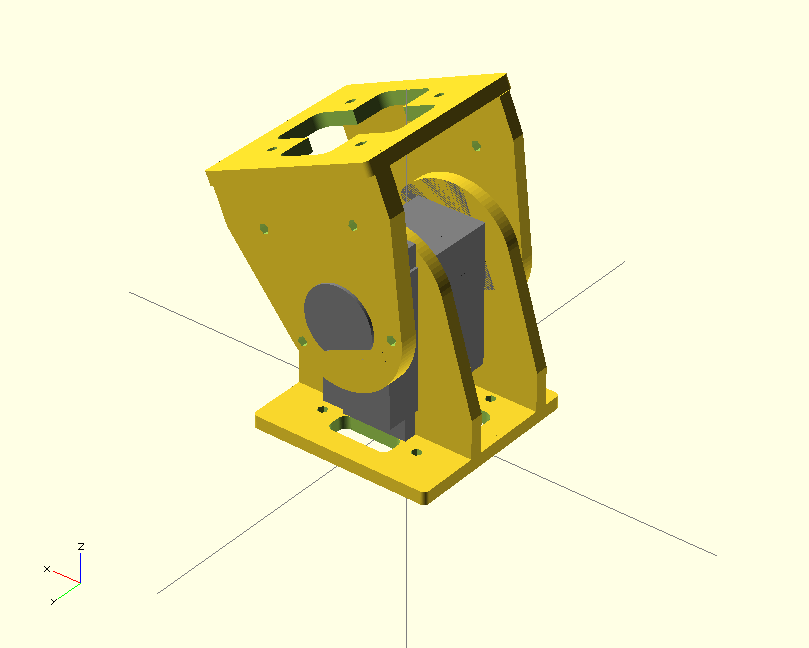
\includegraphics[width=\textwidth]{images/Gait_osc_center_62_5.png}
                \caption{$t = $, $\phi=º$}
                \label{fig:Gait_osc_center_62_5-3}
        \end{subfigure}
        ~
        \begin{subfigure}[b]{0.18\textwidth}
         	   \centering
                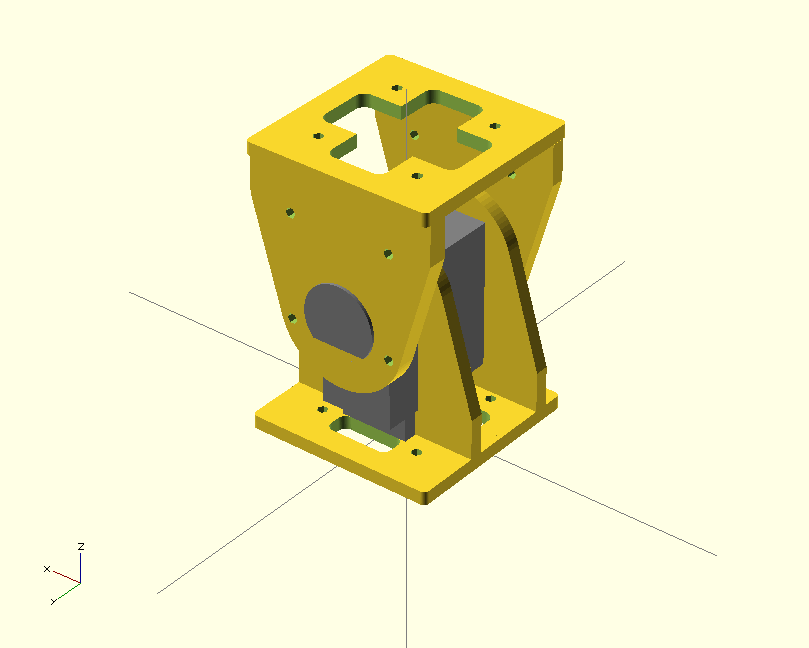
\includegraphics[width=\textwidth]{images/Gait_osc_center_90.png}
                \caption{$t = T$, $\phi=360º$}
                \label{fig:Gait_osc_center_90-3}
        \end{subfigure}
        \caption{Sequence of module oscillation for $A_i = 45º$, $O_i = 0º$}\label{fig:oscillator_center_seq}
\end{figure}

In figure \ref{fig:oscillator_offset_seq} the oscillator has the same amplitude as before, 45º, but the offset has been set to -45º. We can observe that in this case the movement is centered around -45º, with a minimum position at  $ O - A = -90º$ and a maximum one at $O + A = 0º$.\\

\begin{figure}[h]
		\centering
        \begin{subfigure}[b]{0.18\textwidth}
                \centering
                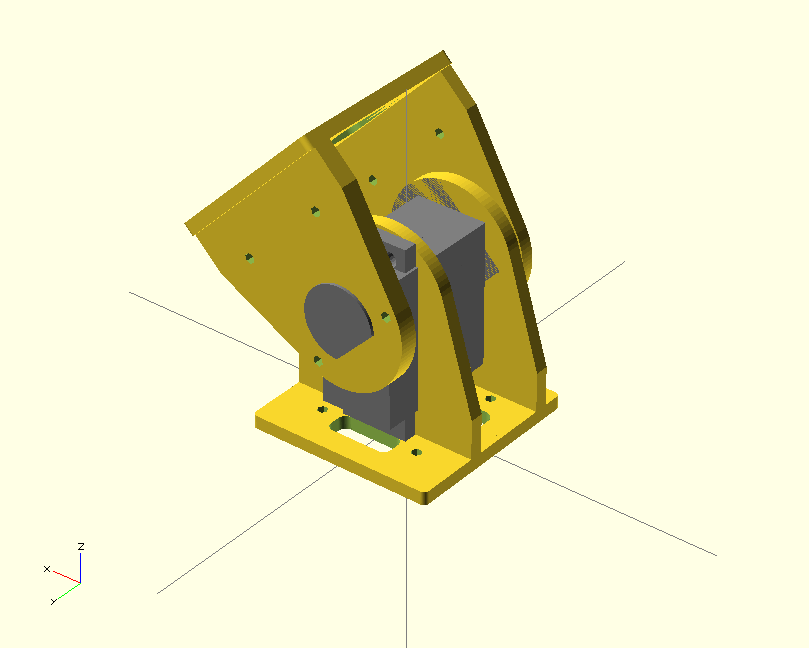
\includegraphics[width=\textwidth]{images/Gait_osc_offset_45.png}
                \caption{$t = 0$, $\phi=0º$}
                \label{fig:Gait_osc_offset_45}
        \end{subfigure}
        ~
        \begin{subfigure}[b]{0.18\textwidth}
                \centering
                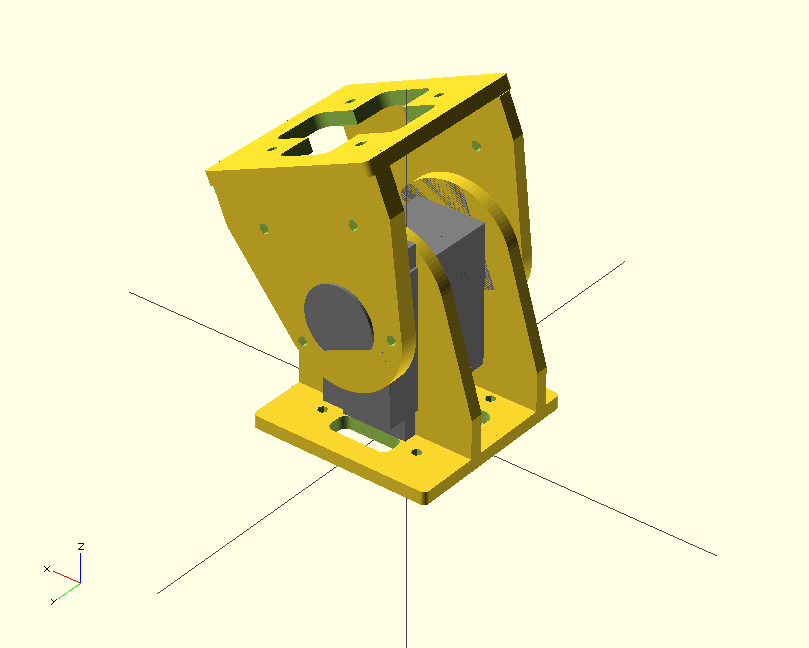
\includegraphics[width=\textwidth]{images/Gait_osc_offset_67_5.png}
                \caption{$t = $, $\phi=º$}
                \label{fig:Gait_osc_offset_67_5}
        \end{subfigure}
        ~
        \begin{subfigure}[b]{0.18\textwidth}
         	   \centering
                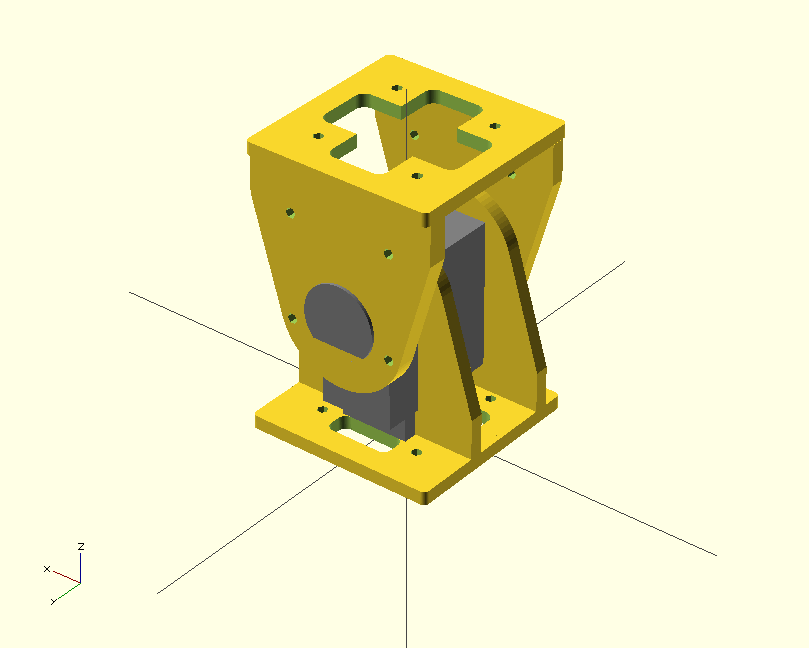
\includegraphics[width=\textwidth]{images/Gait_osc_offset_90.png}
                \caption{$t = \frac{T}{4}$, $\phi=90º$}
                \label{fig:Gait_osc_offset_90}
        \end{subfigure}
        ~
        \begin{subfigure}[b]{0.18\textwidth}
         	   \centering
                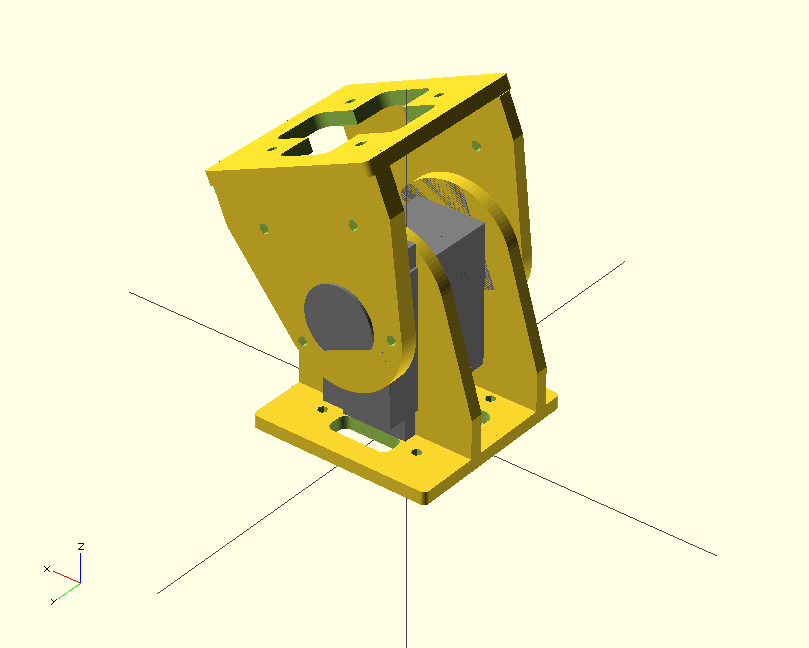
\includegraphics[width=\textwidth]{images/Gait_osc_offset_67_5.png}
                \caption{$t = $, $\phi=º$}
                \label{fig:Gait_osc_offset_67_5-2}
        \end{subfigure}
        ~
        \begin{subfigure}[b]{0.18\textwidth}
         	   \centering
                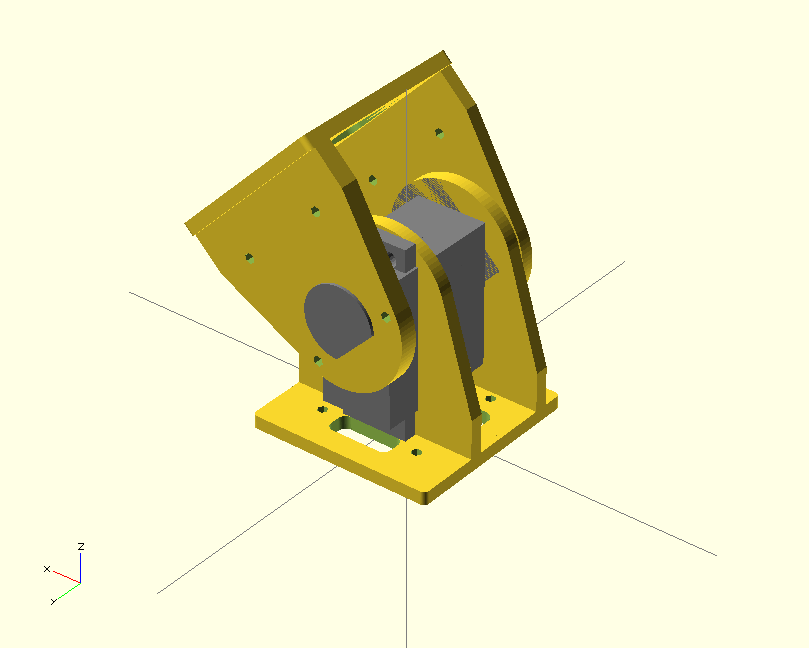
\includegraphics[width=\textwidth]{images/Gait_osc_offset_45.png}
                \caption{$t = \frac{T}{2}$, , $\phi=180º$}
                \label{fig:Gait_osc_offset_45-2}
        \end{subfigure}
        ~
                \begin{subfigure}[b]{0.18\textwidth}
                \centering
                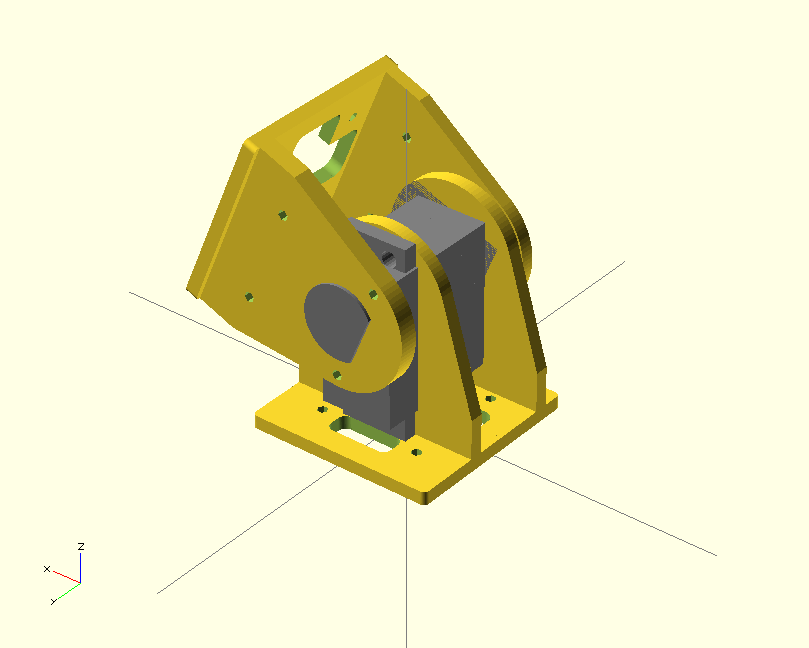
\includegraphics[width=\textwidth]{images/Gait_osc_offset_22_5.png}
                \caption{$t = $, $\phi=º$}
                \label{fig:Gait_osc_offset_22_5-2}
        \end{subfigure}
        ~
        \begin{subfigure}[b]{0.18\textwidth}
                \centering
                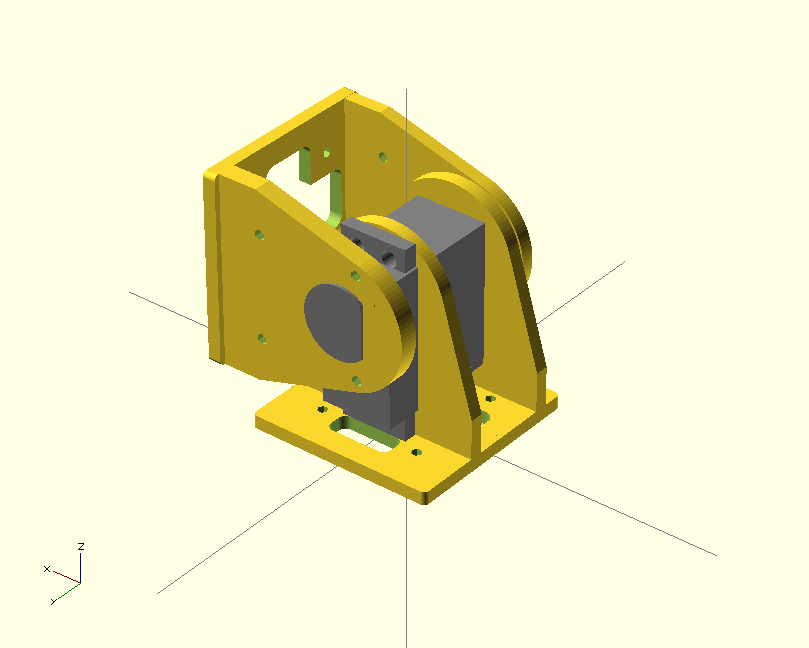
\includegraphics[width=\textwidth]{images/Gait_osc_offset_0.png}
                \caption{$t = \frac{3T}{4}$, $\phi=270º$}
                \label{fig:Gait_osc_offset_0-2}
        \end{subfigure}
        ~
        \begin{subfigure}[b]{0.18\textwidth}
         	   \centering
                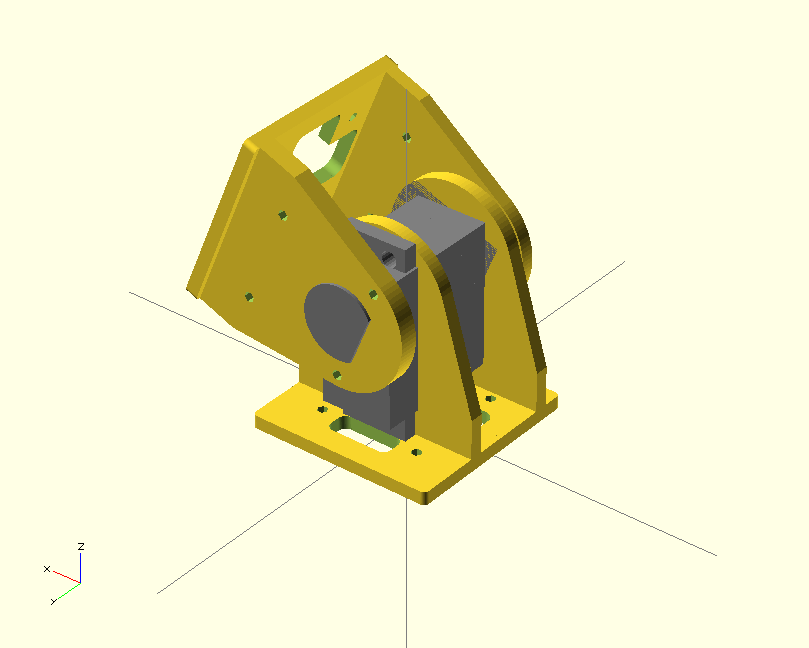
\includegraphics[width=\textwidth]{images/Gait_osc_offset_22_5.png}
                \caption{$t = $, $\phi=º$}
                \label{fig:Gait_osc_offset_22_5-3}
        \end{subfigure}
        ~
        \begin{subfigure}[b]{0.18\textwidth}
         	   \centering
                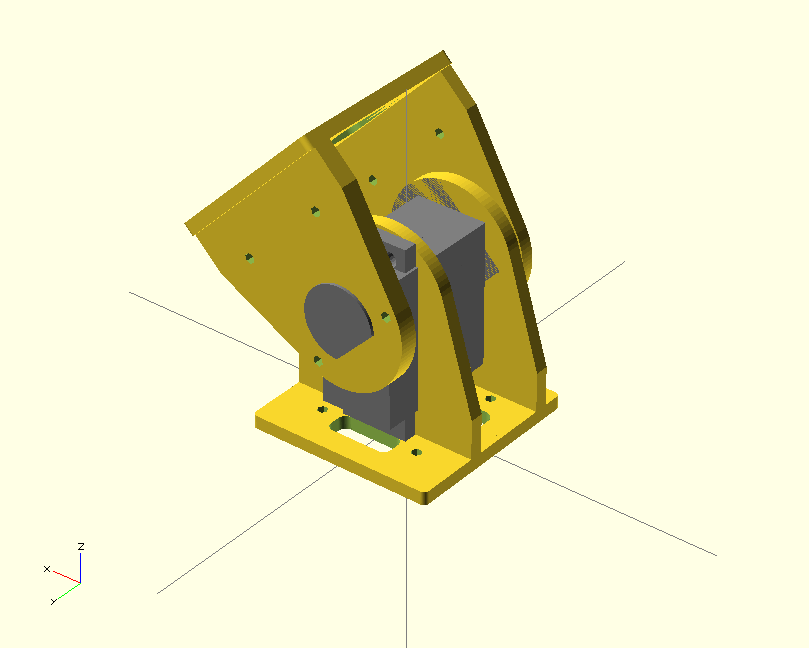
\includegraphics[width=\textwidth]{images/Gait_osc_offset_45.png}
                \caption{$t = T$, $\phi=360º$}
                \label{fig:Gait_osc_offset_45-3}
        \end{subfigure}
        \caption{Sequence of module oscillation for $A_i = 45º$, $O_i = -45º$}\label{fig:oscillator_offset_seq}
\end{figure}

\section{Evolving Gaits}
\label{gaits_evolution}

When the number of modules in the modular robot is high, or the distribution of the modules is complex, setting the parameters of the sinusoidal oscillators by hand becomes an almost impossible task, and the gaits obtained by this method are very far from the optimal ones.\\

As it is very easy to evaluate in simulation how much did a modular robot travell in a certain period of time with a given set of oscillator parameters ($A_i$, $O_i$, $\phi_i$ and T), we can try random values for those parameters and use the ones that yield better gaits. This is the approach taken by the stochastic optimization algorithms, such as simulated annealing, particle swarm optimization or genetic algorithms. Differential evolution, the algorithm used in this thesis for optimizing the oscillator parameters belongs to the later group of stochastic optimization algorithms.\\

\subsection{Differential Evolution}
\label{evolution_DE}
Differential evolution (DE) is a iterative method to optimize a multidimensional real-valued function by keeping a population of candidate solutions that is improved over time using simple arithmetic operations between the individuals of the population. Since it takes few or any assumptions on the function to be optimized, and can search over a large space of candiate solutions, this method is called a metaheuristic method. As a drawback, metaheuristic methods do not ensure a optimal solution, but for many applications the solution obtained with these methods is good enough for meeting the requirements.\\

Differential evolution is inspired by biology and the evolution of living beings, keeping a population of candidate solutions from which only the fittest survive and produce offspring by mixing the candidate solutions, replacing the worst individuals from the population. This way, the population is improved and the parameters to optimize (genotype) are closer to the optimal solution. In order to escape from possible local minima existing in the function to optimize, the concept of random mutation is introduced, so that after a certain number of iterations an individual can have some of its variables randomly modified, in order to create genetic variability in their offspring. The fitness value for indidual is given by the cost function to maximize, that for this thesis is the average speed of the modular robot through the evaluation time. The process finishes when a certain level of fitness is reached (the algorithm as found a ``good enough'' solution) or after a given number of iterations.\\

This algorithm, as opposed to other optimization methods such as Gradient Descend, does not use the gradient of the function for locating the minima/maxima of the function, and therefore does not require the cost function to be differentiable. Furthermore, the cost function is seen as a ``black box'' by the differential evolution algorithm, that uses it to evaluate how good a candidate solution is, and to check whether or not a new candidate obtained by recombination is better than its parents in order to substitute their parents by it on the population, making this algorithm a good choice for a wide range of optimization problems with a cost function difficult to model analitically, such as the gait optimization problem.\\

\subsection{Algorithm}
\label{evolution_algorithm}

Let us have a cost function $J(\theta): \mathbb{R}^n \rightarrow \mathbb{R}$ to maximize and a population of candidates to be the maximum of the function where $x_ \in \mathbb{R}^n$ denotes an individual of that population. The algorithm for Differential Evolution is as follows:\\

\begin{algorithm}
\caption{Differential Evolution algorithm}\label{DE_algorithm}
\begin{algorithmic}[1]
\State Random initialization of all individual x in the population
\While {finalization criteria is not met}
\ForAll{ $x \in \text population$}
	\State Pick three random individuals a, b, c from population different than x
	\State Generate random number $ R \in \{1, \cdots, n\}$, where $n$ is the genotype size
	\State Compute the candidate to be the new position of the individual $y = [ y_1 ~ \cdots ~ y_n ]$ with this procedure:
	\For{ i := 1 to n}
		\State Pick uniformly distributed number $r_i \equiv U(0, 1)$
		\If{ $r_i < CR$ or $i = R$}
		\State $y_i \gets a_i + F \cdot (b_i-c_i)$
		\Else
		\State $y_i \gets x_i$ 
		\EndIf
	\EndFor
	\If{$J(y) > J(x)$}
		\State Replace x with y in the population
	\EndIf
\EndFor
\EndWhile
\State Pick the fittest individual as solution
\end{algorithmic}
\end{algorithm}

Finalization criteria, as explained before, can be either a given number of iterations reached, or that the best individual has a fitness value above a given threshold.\\

Some important parameters that control the behavior of the algorithm are $F \in [0, 2]$, called \emph{differential weight}, that controls the amplification of the differential variation (a value of 0.8 is suggested) , $CR \in [0, 1]$, called \emph{crossover probability}, the probability of a recombination ocurring (a value of 0.9 is suggested) and $NP \geq 4$ , the \emph{population size}.


\subsection{Application to gait optimization}
\label{evolution_gait_opt}

In order to apply this algorithm to the gait optimization problem, a simple sinusoidal contoller was created for the OpenRAVE simulated modular robot. The oscillator parameters ($A_i$, $O_i$, $\phi_i$  for each oscillator, plus the frequency ($f= \frac{1}{T}$) of all of them) are encoded in the genotype of the individual. As the evolutionary optimization library used (ECF, section \ref{software_ECF}) did not support using several gentypes with different limits, the genotype was constraint to have values between $[-1, 1]$ and then later scaled to the suitables ranges for each parameter. In order to avoid collisions between limbs, the ranges for amplitude and offset where constraint to $[0º, 60º]$ for $A_i$ and $[-15º, 15º]$ for $O_i$.\\

\begin{table}[h]
\centering
\begin{tabular}{|c||c|c|} \hline
Symbol & Description & Constraint range \\ \hline \hline
$A_i$ & Amplitude of the ith oscillator & [0, 60] degrees \\ \hline
$O_i$ & Offset of ith oscillator & [-15, 15] degrees \\ \hline
$\phi_i$ & Initial phase of ith oscillator & [0, 360] degrees \\ \hline
$f$ & Frequency of all the oscillators $ f=\frac{1}{T}$ &  [0, 1.5] hz \\ \hline

\end{tabular}
\caption{Values used for gait optimization}
\label{tab:osc_constraints}
\end{table}


For the evaluation of each individual the parameters are extracted from the genome, converted to values within the ranges provided in table \ref{tab:osc_constraints}, and set to the corresponding oscillators. Then, the simulation is run for 30s (simulation time), and the average speed is used as fitness value. Therefore, the cost function used for optimization is:

\begin{equation} \label{eq:cost_function}
J( \vec{A}, \vec{O}, \vec{\Phi}, f) = \frac{\text{Distance travelled}(m)}{\text{Evaluation time}(s)} \qquad \text{where: } 
	\begin{cases}
	\vec{A} = [ A_1 ~ A_2 ~ \cdots ~ A_N] \\
	\vec{O} = [ O_1 ~ O_2 ~ \cdots ~ O_N] \\
	\vec{\Phi} = [ \Phi_1 ~ \Phi_2 ~ \cdots ~ \Phi_N] \\
	\end{cases}
\end{equation}\\

Once a suitable gait has been discovered for a configuration, the parameters are stored in a table for that configuration, similar to a gait table, but with the three oscillator parameters ($A_i$, $O_i$, $\phi_i$)  assigned to their corresponding module ID. The frequency is also extracted and stored in another table, shared by all the configurations, and assigned to the ID of the configuration. This process is repeated for the three configurations to be evaluated on this thesis.\\